\documentclass[12pt, a4paper, english]{article}
\usepackage[top=1.5cm, bottom=2.5cm, left=1cm, right=1cm]{geometry}
\usepackage[utf8]{vietnam}
\usepackage{array}
\usepackage{caption}
% \captionsetup[table]{name=}
\usepackage{biblatex}
\addbibresource{references.bib}
\usepackage{amsmath,amsthm,amsfonts,amssymb,amscd, fancyhdr, color, comment, graphicx, environ}
\usepackage{mathtools}
\usepackage[
  bookmarksopen,
  bookmarksdepth=2,
  breaklinks=true
]{hyperref}
\usepackage{float}
\usepackage{lastpage}
\usepackage[dvipsnames]{xcolor}
\usepackage{xcolor}
\usepackage[framemethod=TikZ]{mdframed}
\usepackage{enumerate}
\usepackage[shortlabels]{enumitem}
\usepackage{fancyhdr}
\usepackage{indentfirst}
\usepackage{listings}
\usepackage{sectsty}
\usepackage{thmtools}
\usepackage{shadethm}
\usepackage{setspace}
\usepackage{footnote}
\usepackage{nicematrix}
\usepackage{multirow}
\usepackage{booktabs}
\usepackage{amsmath,amsxtra,amssymb,latexsym, amscd,amsthm}
\usepackage{import}
\usepackage{graphicx,todo}
\usepackage{xstring}
\usepackage{mathrsfs}
\usepackage{tikz}
\usetikzlibrary{calc,intersections}
\usetikzlibrary{arrows}
\usepackage{tkz-base}
\usepackage{tkz-euclide}
\usepackage{tkz-tab}
\usepackage{import}
\usepackage{multicol}
% \usepackage{listings}
\usepackage{lscape}
\usepackage{booktabs}
\usepackage{tabto}
\usepackage[most]{tcolorbox}
\usepackage{tabularx}
\newcolumntype{C}[1]{>{\centering\arraybackslash}p{#1}}

% \usepackage{mathrsfs}
% \usepackage{newtxmath}
% \usepackage{mathptmx} % dùng để chỉnh font Latex
% \usepackage[math-style=ISO]{unicode-math} % dùng để chỉnh font Latex
% \setmathfont{TeX Gyre Termes Math} % dùng để chỉnh font Latex

%%%%%%%%%%%%%%%%%%%%
% Code setup
\usepackage{fancyvrb} % C++
\usepackage{environ} % added  <<<<<<<<<<<<
\NewEnviron{TCBx}{ % footnotes ouside the box
    \begin{savenotes}
        \begin{tcolorbox}
                \BODY   
        \end{tcolorbox}
    \end{savenotes}}
\hypersetup{
    colorlinks=true,
    linkcolor=blue,
    filecolor=magenta,      
    urlcolor=blue,
}

% Environment setup
\mdfsetup{skipabove=\topskip,skipbelow=\topskip}
\newrobustcmd\ExampleText{%
  An \textit{inhomogeneous linear} differential equation has the form
  \begin{align}
    L[v] = f,
  \end{align}
  where $L$ is a linear differential operator, $v$ is the dependent
  variable, and $f$ is a given non-zero function of the independent
  variables alone.
}
\mdfdefinestyle{theoremstyle}{%
  linecolor=black,linewidth=1pt,%
  frametitlerule=true,%
  frametitlebackgroundcolor=gray!20,
  innertopmargin=\topskip,
}
\mdtheorem[style=theoremstyle]{Problem}{Problem}
\newenvironment{Solution}{\textbf{Solution.}}

\definecolor{codegreen}{rgb}{0,0.6,0}
\definecolor{codegray}{rgb}{0.5,0.5,0.5}
\definecolor{codepurple}{rgb}{0.58,0,0.82}
\definecolor{backcolour}{rgb}{0.95,0.95,0.92}

\lstdefinestyle{mystyle}{
  backgroundcolor=\color{backcolour},   
  commentstyle=\color{codegreen},
  keywordstyle=\color{magenta},
  numberstyle=\tiny\color{codegray},
  stringstyle=\color{codepurple},
  basicstyle=\ttfamily\footnotesize,
  breakatwhitespace=false,         
  breaklines=true,                 
  captionpos=b,                    
  keepspaces=true,                 
  numbers=left,                    
  numbersep=5pt,                  
  showspaces=false,                
  showstringspaces=false,
  showtabs=false,                  
  tabsize=2
}
\lstset{style=mystyle}
%%%%%%%%%%%%%%%%%%%%

%%%%%%%%%%%%%%%%%%%%
% Fill in the appropriate information below
\newcommand{\norm}[1]{\left\lVert#1\right\rVert}     
\newcommand\course{XXXX0000}        % <-- course name   
\newcommand\hwnumber{0}             % <-- homework number
\newcommand\Information{Someone}    % <-- personal information
%%%%%%%%%%%%%%%%%%%%

%%%%%%%%%%%%%%%%%%%%
% Page setup
%---------------
\pagestyle{fancy}
\headheight 35pt
% \lhead{\today}
% \rhead{
\includegraphics[width=2.5cm]{UMT_1.jpg}}
% \lfoot{}
% \pagenumbering{arabic}
% \cfoot{\small\thepage}
% \rfoot{}
\headsep 1.2em
\renewcommand{\baselinestretch}{1.25}
%---------------
\fancyhead{}
\fancyhead[L]{
  \begin{tabular}[c]{@{}c@{}}
    
\includegraphics[width=2.75cm]{Logo/UMT_1.jpg}
  \end{tabular}
  \fontsize{10}{8}\selectfont
  \begin{tabular}[c]{@{}l@{}}
    \textbf{Trường Đại học Quản lý và Công nghệ TP. HCM} \\
    \textbf{Khoa Công nghệ}
  \end{tabular}
}
\fancyhead[R]{
  \begin{tabular}{l}
    \fontsize{10}{8}\selectfont
    \textbf{Phan Vĩnh Tiến}
  \end{tabular}
}
\fancyfoot{}
\fancyfoot[R]{
  {\small\nouppercase{\fontsize{10}{8}\selectfont \textbf{\rightmark}}}}
\fancyfoot[L]{\parbox[t]{0.4\linewidth}{
  {\small\nouppercase{\fontsize{10}{8}\selectfont \textbf{\leftmark}}}}}
\fancyfoot[C]{{\small\nouppercase{\fontsize{10}{8}\selectfont \textbf{Trang {\thepage}/\pageref{LastPage}}}}}
%%%%%%%%%%%%%%%%%%%%

%%%%%%%%%%%%%%%%%%%%
% Tcolorbox
\BeforeBeginEnvironment{tcolorbox}{\savenotes}
\AfterEndEnvironment{tcolorbox}{\spewnotes}
%%%%%%%%%%%%%%%%%%%%

%%%%%%%%%%%%%%%%%%%%
% New definition
\renewcommand{\labelenumi}{\alph{enumi})}
\newcommand{\Z}{\mathbb Z}
\newcommand{\R}{\mathbb R}
\newcommand{\Q}{\mathbb Q}
\newcommand{\NN}{\mathbb N}
\newcommand{\PP}{\mathbb P}
\DeclareMathOperator{\Mod}{Mod} 
\renewcommand\lstlistingname{Algorithm}
\renewcommand\lstlistlistingname{Algorithms}
\def\lstlistingautorefname{Alg.}
\newtheorem*{theorem}{Theorem}
\newtheorem*{lemma}{Lemma}
\newtheorem{case}{Case}
\newcommand{\assign}{:=}
\newcommand{\infixiff}{\text{ iff }}
\newcommand{\nobracket}{}
\newcommand{\backassign}{=:}
\newcommand{\tmmathbf}[1]{\ensuremath{\boldsymbol{#1}}}
\newcommand{\tmop}[1]{\ensuremath{\operatorname{#1}}}
\newcommand{\tmtextbf}[1]{\text{{\bfseries{#1}}}}
\newcommand{\tmtextit}[1]{\text{{\itshape{#1}}}}
%%%%%%%%%%%%%%%%%%%%

%%%%%%%%%%%%%%%%%%%%
\newcommand*{\mkbibnextfootnotetext}[1]{\nextfootnotetext{\blxmkbibnote{foot}{#1}}}
\DeclareCiteCommand{\footcitetext}[\mkbibnextfootnotetext]
  {\usebibmacro{prenote}}
  {\usebibmacro{citeindex}%
    \usebibmacro{cite}}
  {\multicitedelim}
  {\usebibmacro{cite:postnote}}
%%%%%%%%%%%%%%%%%%%%

%%%%%%%%%%%%%%%%%%%% 
% Custom matrix
\makeatletter
\renewcommand*\env@matrix[2][1.0]{%
  \edef\arraystretch{#1}%
  \hskip -\arraycolsep
  \let\@ifnextchar\new@ifnextchar
  \array{#2}
}
\makeatother
%%%%%%%%%%%%%%%%%%%%

%%%%%%%%%%%%%%%%%%%%
% Some definitions
\theoremstyle{definition}
\allowdisplaybreaks
\newtheorem{dinhly}{Định lý}
\newtheorem{dinhnghia}{Định nghĩa}
\newtheorem{vidu}{Ví dụ}
\newtheorem{hequa}{Hệ quả}
\newtheorem{bode}{Bổ đề}
\newtheorem{baitoan}{Bài toán}
\newtheorem{luuy}{Lưu ý}
\newtheorem{nhanxet}{Nhận xét}
%%%%%%%%%%%%%%%%%%%%

%%%%%%%%%%%%%%%%%%%%
% Create files inside Latex file
\begin{filecontents}{references.bib}
  @book{shahriari2021invitation,
    title={An invitation to combinatorics},
    author={Shahriari, Shahriar},
    year={2021},
    publisher={Cambridge University Press}
  }
\end{filecontents}
%%%%%%%%%%%%%%%%%%%%

%%%%%%%%%%%%%%%%%%%%
% Stirling numbers
\newcommand{\genstirlingI}[3]{%
	\genfrac{[}{]}{0pt}{#1}{#2}{#3}%
}
\newcommand{\genstirlingII}[3]{%
	\genfrac{\{}{\}}{0pt}{#1}{#2}{#3}% 
}
\newcommand{\stirlingI}[2]{\genstirlingI{}{#1}{#2}}
\newcommand{\dstirlingI}[2]{\genstirlingI{0}{#1}{#2}}
\newcommand{\tstirlingI}[2]{\genstirlingI{1}{#1}{#2}}
\newcommand{\stirlingII}[2]{\genstirlingII{}{#1}{#2}}
\newcommand{\dstirlingII}[2]{\genstirlingII{0}{#1}{#2}}
\newcommand{\tstirlingII}[2]{\genstirlingII{1}{#1}{#2}}
%%%%%%%%%%%%%%%%%%%%

%%%%%%%%%%%%%%%%%%%% % Indent & Line-spacing
\setlength\parindent{0pt}
\setlist{nolistsep}
\def\multiset#1#2{\ensuremath{\left(\kern-.3em\left(\genfrac{}{}{0pt}{}{#1}{#2}\right)\kern-.3em\right)}}
\usepackage{breakurl}
%%%%%%%%%%%%%%%%%%%%



\begin{document}
  \begin{titlepage}
    \begin{center}
      \fontsize{11}{8}\selectfont \text{BỘ GIÁO DỤC VÀ ĐÀO TẠO} \\
      \fontsize{11}{8}\selectfont \text{TRƯỜNG ĐẠI HỌC QUẢN LÝ VÀ CÔNG NGHỆ THÀNH PHỐ HỒ CHÍ MINH} \\        
      \fontsize{11}{8}\selectfont \textbf{KHOA CÔNG NGHỆ}

      
\includegraphics[width=0.4\textwidth]{Logo/UMT_1.jpg}

      \vspace*{5.5cm}
          
      \Huge
      \textbf{BÁO CÁO BÀI TẬP}
      % \textbf{BÁO CÁO BÀI TẬP
      % %\footnote{\normalsize This template is collected and edited by  Phan Vĩnh Tiến.}\footnote{\normalsize Unless otherwise noted, all the problems are in the \textbf{7th edition} of the book \textit{Discrete Mathematics and Its Applications} - Kenneth H. Rosen.}
      % }
          
      \Large
      TỔ HỢP VÀ LÝ THUYẾT ĐỒ THỊ \& GIẢI TÍCH
          
      \vspace{2cm}

      \Large
      \begin{table}[h]
        \begin{tabular}{rrl}
          \fontsize{12}{8}\selectfont
          % \hspace{5 cm} & Giảng viên:  & PGS. TS. Đỗ Văn Nhơn \\
          % \hspace{5 cm} &              & TS. Nguyễn Tấn Trung \\
          \hspace{2.5 cm} 
          & \textbf{Giảng viên hướng dẫn:}  & ThS. Nguyễn Quản Bá Hồng \\
          \newline
          & \textbf{Sinh viên thực hiện:}   & Phan Vĩnh Tiến -- 2201700177 -- IT2207A \\
        \end{tabular}
      \end{table} 

      \vfill
      \vspace{9cm}
      
      \MakeUppercase{\fontsize{12}{8}\selectfont THÀNH PHỐ HỒ CHÍ MINH, \today}
    \end{center}
  \end{titlepage}
  \newpage

  \tableofcontents
  \newpage

  \section*{Tiến trình}
    \begin{table}[h]
    \centering
    \begin{tabular}{|C{2.5cm}|m{15cm}|}
        \hline
        \bf Tuần & \multicolumn{1}{>{\centering\arraybackslash}m{15cm}|}{\textbf{Bài tập}} \\

        \hline
        1 (06/05) & \ref{pb:w01:01}, \ref{pb:w01:02} \\
        \hline
        2 (13/05) & \ref{pb:w02:01}, \ref{pb:w02:02}, \ref{pb:w02:03}, \ref{pb:w02:04}, \ref{pb:w02:05}, \ref{pb:w02:06}, \ref{pb:w02:07}, \ref{pb:w02:08}b  \\
        \hline
        3 (20/05) &  \\
        \hline
        4 (27/05) &  \\
        \hline
        5 (05/06) &  \\
        \hline
        6 (26/06) &  \\
        \hline
        7 (03/07) &  \\
        \hline
        8 (15/07) &  \ref{pb:w05:01}, \ref{pb:w05:02}, \ref{pb:w05:03}, \ref{pb:w05:04}, \ref{pb:w08:34}, \ref{pb:w08:35}, \ref{pb:w08:36}, \ref{pb:w08:22}, \ref{pb:w08:23}, \ref{pb:w08:24}, \ref{pb:w08:06}, \ref{pb:w08:07}, \ref{pb:w08:08}, \ref{pb:w08:01} \\
        \hline
    \end{tabular}
\end{table}
  \newpage

  \part{Tổ hợp và Lý thuyết đồ thị}
    \textbf{Lời giải đề thi giữa học kỳ: }\url{https://github.com/vinhtienlovemath/PublicDocuments/blob/main/Combinatorics/Midterm/PDF/main.pdf}.
    
    \section{Các phép đếm nâng cao}
      \subsection{Nguyên lý bù trừ}

\begin{dinhly}[Inclusion--exclusion principle]
	\label{thm: inclusion-exclusion: combinatorial version}
	For any $n\in\mathbb{N}^\star$, and any finite sets $A_1,\,\ldots,\,A_n$, one has the identity
	\begin{equation*}
		\left|\bigcup_{i=1}^n A_i\right| = \sum_{i=1}^n |A_i| - \sum_{1\le i < j\le n} |A_i\cap A_j| + \sum_{1\le i < j < k\le n} |A_i\cap A_j\cap A_k| - \cdots + (-1)^{n+1}|A_1\cap\cdots\cap A_n|,
	\end{equation*}
	which can be compactly written as
	\begin{equation*}
		\left|\bigcup_{i=1}^n A_i\right| = \sum_{k=1}^n (-1)^{k+1}\sum_{1\le i_1 < \cdots < i_k\le n} |A_{i_1}\cap\cdots\cap A_{i_k}|,
	\end{equation*}
	or
	\begin{equation*}
		\left|\bigcup_{i=1}^n A_i\right| = \sum_{\varnothing\ne J\subset\{1,\ldots,n\}} (-1)^{|J|+1} \left|\bigcap_{j\in J} A_j\right|.
	\end{equation*}
\end{dinhly}

\begin{dinhly}[Inclusion--exclusion principle in probability]
	\label{thm: inclusion-exclusion: probabilistic version}
	For any $n\in\mathbb{N}^\star$, and for any events $A_1,\,\ldots,\,A_n$ in a \href{https://en.wikipedia.org/wiki/Probability_space}{probability space} $(\Omega,\,{\cal F},\,\mathbb{P})$, in general
	\begin{align*}
		\mathbb{P}\left(\bigcup_{i=1}^n A_i\right) = \sum_{i=1}^n \mathbb{P}(A_i) - \sum_{1 \leq i < j \leq n} \mathbb{P}(A_i\cap A_j) + \sum_{1 \leq i < j < k \leq n} \mathbb{P}(A_i\cap A_j\cap A_k) + \cdots + (-1)^{n-1}\mathbb{P}\left(\bigcap_{i=1}^n A_i\right),
	\end{align*}
	which can be written in closed form as
	\begin{equation}
		\label{inclusion-exclusion: probabilistic version}
		\mathbb{P}\left(\bigcup_{i=1}^n A_i\right) = \sum_{k=1}^n (-1)^{k-1}\sum_{I\subset[n],\,|I| = k} \mathbb{P}(A_I),
	\end{equation}
	where the last sum runs over all subsets $I$ of the indices $1,\,\ldots,\,n$ which contain exactly $k$ elements, and $\displaystyle A_I\coloneqq\bigcap_{i\in I} A_i$ denotes the intersection of all those $A_i$ with index in $I$.
	
	In particular, if the probability of the intersection $A_I$ only depends on the cardinality of $I$, i.e., for every $k\in[n]$, there is an $a_k$ s.t. $a_k = \mathbb{P}(A_I)$ for every $I\in[n]$ with $|I| = k$, then \eqref{inclusion-exclusion: probabilistic version} simplifies to
	\begin{equation*}
		\mathbb{P}\left(\bigcup_{i=1}^n A_i\right) = \sum_{k=1}^n (-1)^{k-1}\binom{n}{k}a_k.
	\end{equation*}
	In addition, if the events $A_i$ are \href{https://en.wikipedia.org/wiki/Independent_and_identically_distributed}{independent \& identically distributed} (i.i.d.), then $\mathbb{P}(A_i) = p$, $\forall i$, and $a_k = p^k$, hence
	\begin{equation*}
		\mathbb{P}\left(\bigcup_{i=1}^n A_i\right) = 1 - (1 - p)^n.
	\end{equation*}
\end{dinhly}

\begin{tcolorbox}[breakable]
    \begin{baitoan}
        \label{pb:w01:01}
        Với $n \in \mathbb{Z^+}$, xét $A_i\,(i = 1,\,2,\,\ldots,\,n)$ là $n$ tập hợp hữu hạn bất kỳ. 
        
        \begin{enumerate}
            \item[(a)] Chứng minh rằng $$\left|\bigcup\limits_{i = 1}^n A_i\right| = \sum\limits_{\substack{T \subseteq \{1,\,2,\,\ldots,\,n\} \\ T \ne \varnothing}} (-1)^{|T| + 1} \left|\bigcap\limits_{i \in T} A_i\right|.$$
            \item[(b)] Chứng minh rằng khi lấy tổng $m < n$ hạng tử đầu tiên của vế phải, nếu $m$ chẵn thì ta có chặn dưới và nếu $m$ lẻ thì ta có chặn trên của $\displaystyle \left|\bigcup\limits_{i = 1}^n A_i\right|$.
        \end{enumerate}
    \end{baitoan}
\end{tcolorbox}

\textbf{Lời giải. }

\begin{enumerate}
    \item[(a)] {
        Trường hợp $n = 1,\,2$, đẳng thức dễ dàng chứng minh.

        Giả sử đẳng thức đúng đến $n = N$, tức ta đã có $$\left|\bigcup\limits_{i = 1}^N A_i\right| = \sum\limits_{\substack{T \subseteq \{1,\,2,\,\ldots,\,N\} \\ T \ne \varnothing}} (-1)^{|T| + 1} \left|\bigcap\limits_{i \in T} A_i\right|.$$

        Ta cần chứng minh đẳng thức cũng đúng với $n = N + 1$, tức cần chứng minh $$\left|\bigcup\limits_{i = 1}^{N+1} A_i\right| = \sum\limits_{\substack{T \subseteq \{1,\,2,\,\ldots,\,N+1\} \\ T \ne \varnothing}} (-1)^{|T| + 1} \left|\bigcap\limits_{i \in T} A_i\right|.$$

        Thật vậy, áp dụng $|A \cup B| = |A| + |B| - |A \cap B|$ và giả thiết quy nạp, ta được
        \begin{align*}
            \left|\bigcup\limits_{i = 1}^{N+1} A_i\right|
            &= \left|\bigcup\limits_{i = 1}^{N} A_i\right| + \left|A_{N+1}\right| - \left|A_{N+1} \cap \left(\bigcup\limits_{i=1}^N A_i\right)\right| \\
            &= \sum\limits_{\substack{T \subseteq \{1,\,2,\,\ldots,\,N\} \\ T \ne \varnothing}} (-1)^{|T| + 1} \left|\bigcap\limits_{i \in T} A_i\right| + \left|A_{N+1}\right| - \left|\bigcup\limits_{i=1}^N\left(A_{N+1} \cap A_i\right)\right|
        \end{align*}

        Nhận xét rằng tập con khác rỗng của $\{1,\,2,\,\ldots,\,N+1\}$ gồm hai loại: 
        \begin{enumerate}
            \item[$\bullet$] các tập con của $\{1,\,2,\,\ldots,\,N\}$, ký hiệu $S_1,\,S_2,\,\ldots,\,S_m$ (không có phần tử thứ $N+1$);
            \item[$\bullet$] tập $\{N+1\}$ và các tập $\{N+1\} \cup S_i$ (có phần tử thứ $N+1$).
        \end{enumerate}

        Suy ra 
        $$\sum\limits_{\substack{T \subseteq \{1,\,2,\,\ldots,\,N+1\} \\ T \ne \varnothing}} (-1)^{|T| + 1} \left|\bigcap\limits_{i \in T} A_i\right| = \sum\limits_{\substack{T \subseteq \{1,\,2,\,\ldots,\,N\} \\ T \ne \varnothing}} (-1)^{|T| + 1} \left|\bigcap\limits_{i \in T} A_i\right| + \left|A_{N+1}\right| + \sum\limits_{\substack{T \subseteq \{N+1\} \cup S_i \\ T \ne \varnothing}} (-1)^{|T| + 1} \left|\bigcap\limits_{i \in T} A_i\right|.$$

        Như vậy ta chỉ cần chứng minh 
        $$\left|\bigcup\limits_{i=1}^N\left(A_{N+1} \cap A_i\right)\right| = -\left(\sum\limits_{\substack{T \subseteq \{N+1\} \cup S_i \\ T \ne \varnothing}} (-1)^{|T| + 1} \left|\bigcap\limits_{i \in T} A_i\right|\right).$$

        Thật vậy, tiếp tục áp dụng giả thiết quy nạp cho vế trái ta được
        \begin{align*}
            \left|\bigcup\limits_{i=1}^N\left(A_{N+1} \cap A_i\right)\right|
            &= \sum\limits_{\substack{T \subseteq \{1,\,2,\,\ldots,\,N\} \\ T \ne \varnothing}} (-1)^{|T| + 1} \left|\bigcap\limits_{i \in T} \left(A_{N+1} \cap A_i\right)\right| \\
            &= -\left(\sum\limits_{\substack{T \subseteq \{1,\,2,\,\ldots,\,N\} \\ T \ne \varnothing}} (-1)^{|T| + 2} \left|\left(\bigcap\limits_{i \in T} A_i\right) \cap A_{N+1}\right|\right) \\
            &= -\left(\sum\limits_{\substack{T' \subseteq \{N+1\} \cup S_i \\ T' \ne \varnothing}} (-1)^{|T'| + 1} \left|\bigcap\limits_{i \in T'} A_i\right|\right).
        \end{align*}

        Như vậy đẳng thức cũng đúng với $n = N+1$. Theo nguyên lý quy nạp toán học, ta có điều phải chứng minh.
    }
    \item[(b)] {
        Đặt $\displaystyle P(n,\,k) = (-1)^{k+1}\sum\limits_{1 \leq i_1 < \cdots < i_k \leq n} \left|\bigcap\limits_{j=1}^k A_{i_j} \right|$ đẳng thức vừa chứng minh có thể được viết lại 

        $$\left|\bigcup\limits_{i = 1}^n A_i\right| = \sum\limits_{i = 1}^n (-1)^{k+1} \sum\limits_{1 \leq i_1 < \cdots < i_k \leq n} \left|\bigcap\limits_{j=1}^k A_{i_j} \right| = \sum\limits_{k = 1}^n P(n,\,k).$$

        Ta sẽ chứng minh với mọi $m \in \mathbb{Z^+},\,m < n$ thì 

        $$\left|\bigcup\limits_{i = 1}^n A_i\right| \leq \sum\limits_{k = 1}^m P(n,\,k) \text{ nếu $m$ lẻ và }\left|\bigcup\limits_{i = 1}^n A_i\right| \geq \sum\limits_{k = 1}^m P(n,\,k) \text{ nếu $m$ chẵn}$$ bằng phương pháp quy nạp toán học.

        Trường hợp $n = 1$, mệnh đề hiển nhiên đúng. Giả sử mệnh đề đúng đến $n = N$, tức ta đã có 
        $$\left|\bigcup\limits_{i = 1}^N A_i\right| \leq \sum\limits_{k = 1}^m P(N,\,k) \text{ nếu $m$ lẻ và }\left|\bigcup\limits_{i = 1}^N A_i\right| \geq \sum\limits_{k = 1}^m P(N,\,k) \text{ nếu $m$ chẵn}.$$

        Ta cần phải chứng minh mệnh đề cũng đúng với $n = N+1$, tức cần chứng minh 
        $$\left|\bigcup\limits_{i = 1}^{N+1} A_i\right| \leq \sum\limits_{k = 1}^m P(N+1,\,k) \text{ nếu $m$ lẻ và }\left|\bigcup\limits_{i = 1}^{N+1} A_i\right| \geq \sum\limits_{k = 1}^m P(N+1,\,k) \text{ nếu $m$ chẵn}.$$

        Thật vậy, áp dụng $|A \cup B| = |A| + |B| - |A \cap B|$, ta được 
        $$\left|\bigcup\limits_{i = 1}^{N+1} A_i\right| = \left|A_{N+1}\right| + \left|\bigcup\limits_{i = 1}^{N} A_i\right| - \left|\bigcup\limits_{i = 1}^{N} (A_{N+1} \cap A_i)\right|.$$

        Xét trường hợp $m$ chẵn, trường hợp $m$ lẻ việc chứng minh hoàn toàn tương tự. Khi $m$ chẵn thì $m-1$ lẻ, áp dụng giả thiết quy nạp ta có 
        $$\left|\bigcup\limits_{i = 1}^{N} A_i\right| \geq \sum\limits_{k = 1}^m P(N,\,k) \text{ và } \left|\bigcup\limits_{i = 1}^{N} (A_{N+1} \cap A_i)\right| \leq \sum\limits_{k = 1}^{m-1} Q(N,\,k),$$
        với $\displaystyle Q(N,\,k) = (-1)^{k+1}\sum\limits_{1 \leq i_1 < \cdots < i_k \leq N} \left|\bigcap\limits_{j=1}^k \left(A_{N+1} \cap A_{i_j}\right)\right| = \displaystyle (-1)^{k+1}\sum\limits_{1 \leq i_1 < \cdots < i_k \leq N} \left|A_{N+1} \cap \left(\bigcap\limits_{j=1}^k A_{i_j}\right)\right|$.

        Suy ra $$\left|\bigcup\limits_{i = 1}^{N+1} A_i\right| \geq \left|A_{N+1}\right| + \sum\limits_{k = 1}^m P(N,\,k) - \sum\limits_{k = 1}^{m-1} Q(N,\,k) = \left|A_{N+1}\right| + P(N,\,1) + \sum\limits_{k = 2}^m\left(P(N,\,k) - Q(N,\,k-1)\right).$$

        Mặt khác
        \begin{align*}
            P(N+1,\,k) 
            &= (-1)^{k+1}\sum\limits_{1 \leq i_1 < \cdots < i_k \leq N+1} \left|\bigcap\limits_{j=1}^k A_{i_j} \right| \\
            &= (-1)^{k+1} \left(\left(\sum\limits_{1 \leq i_1 < \cdots < i_k \leq N} + \sum\limits_{1 \leq i_1 < \cdots < i_k = N+1}\right)\left|\bigcap\limits_{j=1}^k A_{i_j} \right|\right) \\
            &= (-1)^{k+1}\sum\limits_{1 \leq i_1 < \cdots < i_k \leq N}\left|\bigcap\limits_{j=1}^k A_{i_j} \right| + (-1)^{k+1}\sum\limits_{1 \leq i_1 < \cdots < i_{k-1} \leq N}\left|\left(\bigcap\limits_{j=1}^{k-1} A_{i_j}\right) \cap A_{N+1} \right| \\
            &= P(N,\,k) - Q(N,\,k-1)
        \end{align*} và 
        $$\left|A_{N+1}\right| + \displaystyle P(N,\,1) = \left|A_{N+1}\right| + \sum\limits_{1 \leq i \leq N} \left|A_{i}\right| = \sum\limits_{1 \leq i \leq N+1} \left|A_{i}\right| = P(N+1,\,1).$$

        Do đó $\displaystyle \left|\bigcup\limits_{i = 1}^{N+1} A_i\right| \geq P(N+1,\,1) + \sum\limits_{k = 2}^m P(N+1,\,k) = \sum\limits_{k = 1}^m P(N+1,\,k)$. Như vậy đối với trường hợp $m$ chẵn, mệnh đề cũng đúng với $n = N+1$. Theo nguyên lý quy nạp toán học, mệnh đề đúng với mọi $n$ nguyên dương. Hoàn tất chứng minh.
    }
\end{enumerate}

      \subsection{Nguyên lý quy nạp}

% \begin{tcolorbox}[breakable]
%     \begin{baitoan}~
        
%         \begin{enumerate}
%             \item[(a)] {}
%             \item[(b)] {} 
%             \item[(c)] {} 
%             \item[(d)] {} 
%         \end{enumerate}
%     \end{baitoan}
% \end{tcolorbox}

% \textbf{Lời giải. }
      \subsection{Lý thuyết tập hợp}

\begin{tcolorbox}[breakable]
    \begin{baitoan}\label{pb:w02:01}Cho tập hợp $A \subset \mathbb{R}$ thỏa mãn đồng thời

        \begin{enumerate}
            \item[(i)] {$Z \subset A$;}
            \item[(ii)] {$\sqrt{2}+\sqrt{3} \in A$;} 
            \item[(iii)] {$x+y \in A,\,xy \in A$ với mọi $x,\,y \in A$.} 
        \end{enumerate}

        Chứng minh rằng $\dfrac{1}{\sqrt{2}+\sqrt{3}} \in A$.
    \end{baitoan}
\end{tcolorbox}

\textbf{Lời giải. }

Vì $\sqrt{2}+\sqrt{3} \in A$, theo (iii) ta có $(\sqrt{2}+\sqrt{3})^2 \in A \iff 5+2\sqrt{6} \in A \iff 2\sqrt{6} \in A$.

Suy ra $2\sqrt{6}\left(\sqrt{2}+\sqrt{3}\right) \in A$ hay $4\sqrt{3} + 6\sqrt{2}\in A$. Kéo theo $\dfrac{1}{\sqrt{2} + \sqrt{3}} = \sqrt{3} - \sqrt{2} = 5(\sqrt{3}+\sqrt{2}) - (4\sqrt{3} + 6\sqrt{2}) \in A$.


      \subsection{Quy tắc đếm}

% \begin{tcolorbox}[breakable]
%     \begin{baitoan}
%         Cho $n\in\mathbb{Z^+}$. Chứng minh rằng số cách khác nhau để đặt đúng đắn $n$ dấu ngoặc mở và $n$ dấu ngoặc đóng bằng số Catalan thứ $n$ $$C_n = \dfrac{1}{n+1}{2n \choose n} = \dfrac{(2n)!}{n!(n+1)!}.$$
%     \end{baitoan}
% \end{tcolorbox}

% \textbf{Lời giải. }


\begin{tcolorbox}[breakable]
    \begin{baitoan}\label{pb:w02:02}
        Cho $m,\,n \in \mathbb{Z^+},\,2m \leq n$. Đếm số các dãy $a_1,\,a_2,\,\ldots,\,a_n$ chứa $m$ số 0 và $n-m$ số 1, thỏa mãn không có hai phần tử nào kề nhau đều là số 0.
    \end{baitoan}
\end{tcolorbox}

\textbf{Lời giải. }Xếp $m$ số 0 thành hàng ngang, khi đó sẽ có $m-1$ khoảng trống ở giữa (cần chèn vào tối thiểu một số 1) và 2 khoảng trống ở hai đầu. Như vậy số dãy thỏa mãn chính là số nghiệm nguyên của phương trình $a_1 + a_2 + \cdots + a_{m+1} = n-m$, với $a_1,\,a_{m+1} \geq 0$ và $a_i \geq 1\,(2 \leq i \leq m)$. Đặt $b_1 = a_1 + 1,\,b_{m+1}=a_{m+1}+1$ thì ta cần tìm số nghiệm nguyên dương của phương trình $b_1 + a_2 + \cdots + a_m + b_{m+1} = n - m + 2$. Theo bài toán chia kẹo Euler, phương trình có tất cả $\displaystyle {n-m+1 \choose m}$ cách, cũng là số các dãy $a_1,\,a_2,\,\ldots,\,a_n$ cần tìm.

\begin{tcolorbox}[breakable]
    \begin{baitoan}\label{pb:w02:03}
        Đặt $f(n)$ là số tập con của $[n]$. Chứng minh rằng $f(n) = 2^n$ với mọi $n$ nguyên dương.
    \end{baitoan}
\end{tcolorbox}

\textbf{Lời giải. }Trường hợp $n=1$, có hai tập con của $[1]$ là $\varnothing,\,\{1\}$ nên $f(1) = 2^1$.

Giả sử mệnh đề đúng tới $n = N$, tức ta đã có $f(N) = 2^N$. Xét các tập con của $[N+1]$, có hai loại
\begin{enumerate}
    \item[$\bullet$] các tập con của $[N]$ (không chứa phần tử $N+1$), có $2^N$ tập;
    \item[$\bullet$] các tập hợp là hợp của $\{N+1\}$ và từng tập con của $[N]$, cũng có $2^N$ tập.
\end{enumerate}

Như vậy $f(N+1) = 2^N + 2^N = 2^{N+1}$ nên mệnh đề cũng đúng với $n = N+1$. Theo nguyên lý quy nạp toán học, ta có điều phải chứng minh.

\begin{tcolorbox}[breakable]
    \begin{baitoan} \label{pb:w05:04}
        Giả sử rằng $n \in \mathbb{Z^+}$ người đưa $n$ chiếc mũ của họ cho mỗi người kiểm tra mũ. Đặt $f(n)$ là số cách trả lại các chiếc mũ, sao cho mỗi người có đúng 1 mũ và không ai nhận lại mũ của họ lúc ban đầu.

        \begin{enumerate}
            \item[(a)] Chứng minh rằng $\displaystyle f(n) = n! \sum\limits_{i=0}^n \dfrac{(-1)^i}{i!}$ với mọi số nguyên dương $n$.
            \item[(b)] Chứng minh rằng $f(n)$ là số nguyên gần nhất với $\dfrac{n!}{\mathrm{e}}$.
        \end{enumerate}
    \end{baitoan}
\end{tcolorbox}

\textbf{Lời giải. }

\begin{enumerate}
    \item[(a)] {
        Khi $n = 1$ thì $f(1) = 0$ (không có cách nào vì một người không thể nhận mũ của chính họ). Khi $n = 2$ thì $f(2) = 1$ (có duy nhất một cách trả lại các chiếc mũ thỏa mãn là đổi mũ cho nhau). Khi $n = 3$ thì $f(3) = 2$ (xét 3 người là $A,\,B,\,C$; giả sử $A$ nhận lại mũ của $B$, $B$ có thể nhận lại mũ của $A$ hoặc $C$, nhưng $B$ chỉ có thể nhận lại mũ của $C$ để $C$ không nhận lại mũ của chính mình, nên trường hợp này có 1 cách; tương tự nếu giả sử $A$ nhận lại mũ của $C$ thì cũng sẽ có 1 cách; như vậy tổng tất cả có 2 cách).

        Ta có nhận xét sau (\href{https://en.wikipedia.org/wiki/Derangement}{derangement}, \parencite{nqbh-combinatorics}): mỗi người có thể nhận được bất kỳ chiếc mũ nào trong số $n - 1$ chiếc mũ không phải của mình. Gọi chiếc mũ mà người $P_1$ nhận được là $h_i$ và xét đến chủ sở hữu của $h_i$: $P_i$ nhận được mũ của $P_1$, $h_1$ hoặc 1 chiếc mũ khác. Theo đó, bài toán chia thành 2 trường hợp có thể xảy ra:
        \begin{itemize}
            \item $P_i$ nhận được 1 chiếc mũ khác với $h_1$. Trường hợp này tương đương với việc giải bài toán với $n - 1$ người và $n - 1$ chiếc mũ vì đối với mỗi $n - 1$ người ngoài $P_1$ thì có đúng $1$ chiếc mũ trong số $n - 1$ chiếc mũ còn lại mà họ không được nhận (đối với bất kỳ $P_j$ nào ngoài $P_i$, chiếc mũ không được nhận là $h_j$, trong khi đối với $P_i$ thì là $h_1$). Một cách khác để thấy điều này là đổi tên $h_1$ thành $h_i$, trong đó sự sắp xếp rõ ràng hơn: đối với bất kỳ $j$ nào từ $2$ đến $n$, $P_j$ không thể nhận được $h_j$.
            \item $P_i$ nhận được $h_1$. Trong trường hợp này, bài toán được rút gọn thành $n - 2$ người và $n - 2$ mũ, vì $P_1$ nhận được mũ của $h_i$ và $P_i$ nhận được mũ của $h_1$, về cơ bản là loại cả hai ra khỏi việc xem xét thêm.
        \end{itemize}

        Đối với mỗi $n - 1$ mũ mà $P_1$ có thể nhận được, số cách mà $P_2,\,\ldots,\,P_n$ có thể nhận được mũ là tổng số đếm của 2 trường hợp. Từ đây ta có
        \begin{equation*}
            f(1) = 0,\,f(2) = 1,\,f(n) = (n - 1)(f(n - 1) + f(n - 2)),\,\forall n\in\mathbb{Z^+},\,n\geq 3.
        \end{equation*}         

        Từ công thức truy hồi trên, ta có $f(n) - nf(n-1) = -f(n-1) + (n-1)f(n-2)$ nên truy hồi ngược về thì $f(n) - nf(n-1) = (-1)^{n-2}\left(f(2) - f(1)\right) = (-1)^n,\,\forall n\in \mathbb{Z^+},\,n\geq 2$. Suy ra $\dfrac{f(n)}{n!} = \dfrac{f(n-1)}{(n-1)!} + \dfrac{(-1)^n}{n!}$, truy hồi ngược về thì được $\displaystyle\dfrac{f(n)}{n!} = \dfrac{f(1)}{1!} + \sum\limits_{i=2}^n \dfrac{(-1)^i}{i!} = \sum\limits_{i=0}^n \dfrac{(-1)^i}{i!}$. Như vậy $\displaystyle f(n) = n! \sum\limits_{i=0}^n \dfrac{(-1)^i}{i!}$ với mọi số nguyên dương $n$.
    }
    \item[(b)] Theo công thức khai triển chuỗi Maclaurin của hàm số $\mathrm{e}^x$ tại $x=-1$, ta có $$\left|\dfrac{n!}{\mathrm{e}} - f(n)\right| = \left|n! \sum\limits_{i=0}^\infty \dfrac{(-1)^i}{i!} - n! \sum\limits_{i=0}^n \dfrac{(-1)^i}{i!}\right| = \left|n!\sum\limits_{i=n+1}^\infty \dfrac{(-1)^i}{i!}\right|.$$
    
    \textbf{Trường hợp 1. }$n$ chẵn. Khi đó $$n!\sum\limits_{i=n+1}^\infty \dfrac{(-1)^i}{i!} = -\dfrac{1}{n+1} +\dfrac{1}{(n+1)(n+2)} -\dfrac{1}{(n+1)(n+2)(n+3)} +\cdots$$ Vì $-\dfrac{1}{(n+1)\cdots(n+2k-1)}+\dfrac{1}{(n+1)\cdots(n+2k-1)(n+2k)} = \dfrac{-n-2k+1}{(n+1)\cdots(n+2k-1)(n+2k)} < 0$ nên $\displaystyle n!\sum\limits_{i=n+1}^\infty \dfrac{(-1)^i}{i!} < 0$. Mặt khác, vì $\dfrac{1}{(n+1)\cdots(n+2k)}-\dfrac{1}{(n+1)\cdots(n+2k-1)(n+2k+1)} = \dfrac{n+2k}{(n+1)\cdots(n+2k-1)(n+2k+1)} > 0$ nên $\displaystyle n!\sum\limits_{i=n+1}^\infty \dfrac{(-1)^i}{i!} > -\dfrac{1}{n+1}$. Từ đó suy ra $-\dfrac{1}{n+1} < \displaystyle n!\sum\limits_{i=n+1}^\infty \dfrac{(-1)^i}{i!} < 0$.

    \textbf{Trường hợp 2. }$n$ lẻ. Bằng việc ghép cặp tương tự trường hợp trên, ta chứng minh được $0 < \displaystyle n!\sum\limits_{i=n+1}^\infty \dfrac{(-1)^i}{i!} < \dfrac{1}{n+1}$.

    Như vậy trong mọi trường hợp thì $\displaystyle \left|n!\sum\limits_{i=n+1}^\infty \dfrac{(-1)^i}{i!}\right| < \dfrac{1}{n+1}$. Do đó $\left|\dfrac{n!}{\mathrm{e}} - f(n)\right| < \dfrac{1}{n+1} \leq \dfrac{1}{2}$ với mọi số nguyên dương $n$ nên $f(n)$ là số nguyên gần nhất với $\dfrac{n!}{\mathrm{e}}$.
\end{enumerate}

\begin{tcolorbox}[breakable]
    \begin{baitoan}\label{pb:w05:03}
        Cho số nguyên dương $n$. Đặt $f(n)$ là số các tập con của $[n]$ không chứa bất kỳ hai số nguyên dương liên tiếp nào.

        \begin{enumerate}
            \item[(a)] Tính $f(1),\,f(2),\,f(3),\,f(4)$.
            \item[(b)] Chứng minh rằng $f(n) = f(n-1)+f(n-2)$ với mọi $n$ nguyên dương, $n \geq 3$.
            \item[(c)] Chứng minh rằng $f(n) = \dfrac{1}{\sqrt{5}}\left(\tau^{n+2} - \overline{\tau}^{n+2}\right)$, với $\tau = \dfrac{1+\sqrt{5}}{2},\,\overline{\tau} = \dfrac{1-\sqrt{5}}{2}$.
        \end{enumerate}
    \end{baitoan}
\end{tcolorbox}

\textbf{Lời giải. }Gọi $S_n$ là tập hợp các tập con của $[n]$ không chứa bất kỳ hai số nguyên dương liên tiếp nào.

\begin{enumerate}
    \item[(a)] {
        $S_1 = \left\{\varnothing,\,\{1\}\right\}$ nên $f(1) = 2$;

        $S_2 = \left\{\varnothing,\,\{1\},\,\{2\}\right\}$ nên $f(2) = 3$;

        $S_3 = \left\{\varnothing,\,\{1\},\,\{2\},\,\{3\},\,\{1,\,3\}\right\}$ nên $f(3) = 5$;

        $S_4 = \left\{\varnothing,\,\{1\},\,\{2\},\,\{3\},\,\{4\},\,\{1,\,3\},\,\{1,\,4\},\,\{2,\,4\}\right\}$ nên $f(4) = 8$.
    }
    \item[(b)] {
        Ta phân $S_n$ thành hai tập:
        \begin{enumerate}
            \item[$\bullet$] tập những tập con của $[n]$ không chứa phần tử $n$: các tập như vậy chính là các tập con của $[n-1]$, nên sẽ có tất cả $f(n-1)$ tập.
            \item[$\bullet$] tập những tập con của $[n]$ có chứa phần tử $n$: các tập như vậy sẽ không chứa phần tử $n-1$, nên sẽ là các tập con của $[n-2]$ hợp với tập $\{n\}$, nên sẽ có tất cả $f(n-2)$ tập. 
        \end{enumerate}

        Như vậy $f(n) = f(n-1) + f(n-2)$.
    }
    \item[(c)] {
        Xét phương trình đặc trưng $\tau^2 = \tau + 1$, phương trình có nghiệm $\tau = \dfrac{1+\sqrt{5}}{2}$ và $\overline{\tau} = \dfrac{1-\sqrt{5}}{2}$.

        Suy ra $f(n) = A\cdot \tau^n + B\cdot \overline{\tau}^n,\,\forall n\in \mathbb{Z^+}$. Vì $A\cdot \tau + B\cdot \overline{\tau} = f(1) = 2$ và $A\cdot \tau^2 + B\cdot \overline{\tau}^2 = f(2) = 3$, nên $A = \dfrac{5+3\sqrt{5}}{10}$ và $B = \dfrac{5-3\sqrt{5}}{10}$. Suy ra $f(n) = \dfrac{5+3\sqrt{5}}{10} \cdot \tau^n + \dfrac{5-3\sqrt{5}}{10} \cdot \overline{\tau}^n = \dfrac{1}{\sqrt{5}}\left(\tau^{n+2} - \overline{\tau}^{n+2}\right)$.
    }
\end{enumerate}
      \subsection{Các số Stirling}
\begin{dinhnghia}[Stirling numbers of the 2nd kind]\label{def: stirling 2}
    Let $s,\,t\in\mathbb{N}$. We define $\displaystyle\stirlingII{s}{t}$ to be the number of ways of putting $s$ distinct balls into $t$ identical boxes with at least 1 ball per box. Equivalently, $\displaystyle\stirlingII{s}{t}$ is the number of ways of partitioning a set of $s$ elements, i.e.,
\begin{equation*}
    [s] = \left\{\begin{split}
        &\{1,\,2,\ldots,\,s\}&&\mbox{if } s > 0,\\
        &[0] = \varnothing&&\mbox{if } s = 0.
    \end{split}\right.
\end{equation*}
into $t$ nonempty parts. $\displaystyle\stirlingII{s}{t}$ is called a {\rm Stirling number of the 2nd kind} (some denote the Stirling numbers of the 2nd kind by $S(s,\,t)$ or $s_2(s,\,t)$).
\end{dinhnghia}

\begin{dinhly}[\parencite{shahriari2021invitation}, Thm. 6.9, p. 198]\label{thm: stirling 2: multiset} 
    Let $s,\,t\in\mathbb{N}$, and let $R = \{\infty\cdot U_1,\,\infty\cdot U_2,\,\ldots,\,\infty\cdot U_t\}$ be a multiset with $t$ types of elements, each with an infinite repetition number. Then the following numbers are equal: (a) The number of ways of placing $s$ distinct balls into $t$ nonempty distinct boxes. (b) The number of $s$-permutations of $R$ that contain each of $U_1,\,\ldots,\,U_t$ at least once. (c) $\displaystyle t!\cdot \stirlingII{s}{t}$.
\end{dinhly}

\begin{tcolorbox}[breakable]
    \begin{baitoan}\label{pb:w05:02}
        Cho $n,\,k\in \mathbb{Z^+}$ và $n \geq k$. Mỗi lần mở ứng dụng ngôn ngữ yêu thích, 1 quảng cáo được chọn ngẫu nhiên trong số $k$ lựa chọn có thể xuất hiện. Giả sử thuật toán có khả năng chọn bất kỳ quảng cáo nào ở mỗi lần là như nhau (uniformly distributed). Tính xác suất sau $n$ lần mở ứng dụng bạn xem đúng $k$ quảng cáo.
    \end{baitoan}
\end{tcolorbox}

\textbf{Lời giải 1. }Ở mỗi lượt xem có $k$ cách chọn quảng cáo, nên trong $n$ lượt xem có tất cả $k^n$ cách chọn quảng cáo, hay $|\Omega| = k^n$.

Đặt $A$ là biến cố ``sau $n$ lần mở ứng dụng bạn xem đúng $k$ quảng cáo'', khi đó số trường hợp thuận lợi của $A$ cũng chính là số cách phân hoạch $n$ lượt xem phân biệt vào $k$ loại quảng cáo phân biệt. Theo định lý \ref{thm: stirling 2: multiset}, ta có $\displaystyle |A| = k! \cdot \stirlingII{n}{k}$.

Như vậy xác suất sau $n$ lần mở ứng dụng xem đúng $k$ quảng cáo là $$\mathbb{P}(A) = \dfrac{|A|}{|\Omega|} = \dfrac{(k-1)!}{k^{n-1}}\stirlingII{n}{k}.$$

\textbf{Lời giải 2. }Đặt $A$ là biến cố ``sau $n$ lần mở ứng dụng bạn xem đúng $k$ quảng cáo'', $A_i$ là biến cố ``sau $n$ lần mở ứng dụng không xem được quảng cáo thứ $i$'' (với $i = 1,\,2,\,\ldots,\,k$). Ta có 
$$\mathbb{P}(A) = 1 - \mathbb{P}(\overline{A}) = 1 - \mathbb{P}\left(\bigcup_{i=1}^k A_i\right),$$
trong đó $\displaystyle\mathbb{P}(\overline{A}) = \mathbb{P}\left(\bigcup_{i=1}^k A_i\right)$ là xác suất để sau $n$ lần mở ứng dụng chưa xem được ít nhất một quảng cáo.

Theo định lý \ref{thm: inclusion-exclusion: probabilistic version}, ta có $$\mathbb{P}\left(\bigcup_{i=1}^k A_i\right) = \sum_{m=1}^k (-1)^{m-1}\sum_{1 \leq i_1 < i_2 < \ldots < i_m \leq k} \mathbb{P}\left(\bigcap_{j=1}^m A_{i_j}\right).$$

Ta có 
\begin{itemize}
    \item $\mathbb{P}(A_i)$: xác suất sau $n$ lần mở ứng dụng không xem được quảng cáo thứ $i$; trong mỗi lượt xem quảng cáo, xác suất không xem được quảng cáo thứ $i$ là $1 - \dfrac{1}{k} = \dfrac{k-1}{k}$, do các lần xem là độc lập nên $$\mathbb{P}(A_i) = \left(\dfrac{k-1}{k}\right)^n,$$ có tất cả $\displaystyle{k \choose 1}$ biến cố $A_i$ như vậy.
    \item $\mathbb{P}(A_i \cap A_j)\,(i < j)$: xác suất sau $n$ lần mở ứng dụng không xem được quảng cáo thứ $i$ và thứ $j$; trong mỗi lượt xem quảng cáo, xác suất không xem được quảng cáo thứ $i$ và thứ $j$ là $1 - \dfrac{2}{k} = \dfrac{k-2}{k}$, nên $$\mathbb{P}(A_i \cap A_j) = \left(\dfrac{k-2}{k}\right)^n,$$ có tất cả $\displaystyle{k \choose 2}$ biến cố $A_i \cap A_j$ như vậy.
    \item Tổng quát, $\displaystyle\mathbb{P}\left(\bigcap_{j=1}^m A_{i_j}\right)$: xác suất sau $n$ lần mở ứng dụng không xem được quảng cáo thứ $i_1,\,i_2,\,\ldots,\,i_m$, tương tự trên ta có $$\displaystyle\mathbb{P}\left(\bigcap_{j=1}^m A_{i_j}\right) = \left(\dfrac{k-m}{k}\right)^n,$$ có tất cả $\displaystyle{k \choose m}$ biến cố $\displaystyle \bigcap_{j=1}^m A_{i_j}$ như vậy.
\end{itemize}

Suy ra $$\mathbb{P}\left(\bigcup_{i=1}^k A_i\right) = \sum_{m=1}^k (-1)^{m-1}{k \choose m}\left(\dfrac{k-m}{k}\right)^n.$$

Như vậy xác suất cần tìm sẽ là $$\mathbb{P}(A) = 1 - \sum_{m=1}^k (-1)^{m-1}{k \choose m}\left(\dfrac{k-m}{k}\right)^n = \sum_{m=0}^k (-1)^{m}{k \choose m}\left(\dfrac{k-m}{k}\right)^n.$$

\begin{tcolorbox}[breakable]
    \begin{baitoan}\label{pb:w05:01}
        Cho $n,\,k\in \mathbb{Z^+}$ và $n \geq k$. Mỗi lần mở ứng dụng ngôn ngữ yêu thích, 1 quảng cáo được chọn ngẫu nhiên trong số $k$ lựa chọn có thể xuất hiện. Giả sử thuật toán có khả năng chọn bất kỳ quảng cáo nào ở mỗi lần là như nhau (uniformly distributed). Tính xác suất bạn cần đúng $n$ lần để xem tất cả $k$ quảng cáo.
    \end{baitoan}
\end{tcolorbox}

Để cần đúng $n$ lần để xem hết tất cả $k$ quảng cáo thì phải thỏa mãn hai điều kiện:
\begin{itemize}
    \item sau $n$ lần mở, tất cả $k$ quảng cáo được xem ít nhất 1 lần;
    \item sau $n-1$ lần mở, chỉ xem đúng $k-1$ quảng cáo.
\end{itemize}

\textbf{Lời giải 1. }Theo bài toán \ref{pb:w05:02}, số cách chọn để sau $n-1$ lần mở xem đúng $k-1$ quảng cáo bằng $\displaystyle (k-1)! \cdot \stirlingII{n-1}{k-1}$.

Chọn $k-1$ quảng cáo trong $k$ quảng cáo để xuất hiện trong $n-1$ lần xem đầu tiên, có $\displaystyle{k \choose k-1}$ cách; chọn quảng cáo còn lại để xuất hiện trong lần xem cuối, có 1 cách. 

Do đó tổng số cách chọn $k$ quảng cáo thỏa mãn đề bài bằng $\displaystyle {k \choose k-1} \cdot (k-1)! \cdot \stirlingII{n-1}{k-1}$, như vậy xác suất sẽ bằng $$\dfrac{\displaystyle{k \choose k-1}(k-1)!}{k^n}\stirlingII{n-1}{k-1} = \dfrac{(k-1)!}{k^{n-1}}\stirlingII{n-1}{k-1}.$$

\textbf{Lời giải 2. }Nhận xét rằng, để trong $n$ lần xem đúng $k$ quảng cáo có hai trường hợp
\begin{itemize}
    \item trong $n-1$ lần đầu đã xem hết quảng cáo: tức trong $n-1$ lần xem đúng $k$ quảng cáo;
    \item trong $n-1$ lần đầu chưa xem hết quảng cáo: tức trong $n-1$ lần xem đúng $k-1$ quảng cáo, lần thứ $n$ xem quảng cáo còn lại (ta cần tính xác suất của trường hợp này).
\end{itemize}

Theo bài toán \ref{pb:w05:02}, xác suất để trong $n$ lần xem đúng $k$ quảng cáo bằng $\displaystyle\sum_{m=0}^k (-1)^{m}{k \choose m}\left(\dfrac{k-m}{k}\right)^n$ và xác suất để trong $n-1$ lần xem đúng $k$ quảng cáo bằng $\displaystyle\sum_{m=0}^k (-1)^{m}{k \choose m}\left(\dfrac{k-m}{k}\right)^{n-1}$. Khi đó xác suất cần tính sẽ bằng 

$$\sum_{m=0}^k (-1)^{m}{k \choose m}\left(\dfrac{k-m}{k}\right)^n - \sum_{m=0}^k (-1)^{m}{k \choose m}\left(\dfrac{k-m}{k}\right)^{n-1} = \sum_{m=0}^k (-1)^{m+1}{k \choose m}\dfrac{m(k-m)^{n-1}}{k^n}.$$



      \subsection{Số Bell}
      \subsection{Số Catalan}
% \begin{tcolorbox}[breakable]
%     \begin{baitoan}\label{pb:w08:33}
%         Chứng minh rằng (a) Số Catalan thỏa mãn quan hệ truy hồi
%         \begin{align}
%             C_0 = 1,\ C_n &= \sum_{i=1}^n C_{i-1}C_{n-i},\ \forall n\in\mathbb{N}^\star,\label{Catalan: recurrence}\\
%             C_0 = 1,\ C_n &= \frac{2(2n - 1)}{n + 1}C_{n-1},\ \forall n\in\mathbb{N}^\star.\nonumber
%         \end{align}
%         (b) Một cách tiệm cận, số Catalan xấp xỉ
%         \begin{equation*}
%             C_n\sim\frac{4^n}{n^{\frac{3}{2}}\sqrt{\pi}},\ \forall n\in\mathbb{N}^\star,
%         \end{equation*}
%         nói cách khác $\lim_{n\to\infty} \dfrac{C_nn^{\frac{3}{2}}\sqrt{\pi}}{4^n} = 1$.
%     \end{baitoan}
% \end{tcolorbox}

% \textbf{Lời giải. }
      \subsection{Số Fibonacci \& Lucas}
      \subsection{Đếm bằng hai cách}
      \subsection{Quan hệ hồi quy}

\begin{tcolorbox}[breakable]
    \begin{baitoan}[\cite{shahriari2021invitation}, P1.3.3, p. 22]\label{pb:w08:34}
        Giả sử $h_n$ biểu thị số cách phủ mảng $2\times n$ bằng $1\times 2$ domino. Tìm $h_1,h_2,h_3$, \& 1 quan hệ đệ quy cho $h_n$. Sử dụng chúng để tìm $h_8$.
    \end{baitoan}
\end{tcolorbox}

\textbf{Lời giải. }Với $n = 1$ có 1 cách nên $h_1=1$. Với $n=2$ có 2 cách (đặt 2 miếng domino cùng dọc, hoặc cùng ngang). Với $n\geq 2$, nếu ô đầu tiên là domino dọc thì còn lại mảng $2 \times (n-1)$ nên có $h_{n-1}$ cách; nếu ô đầu tiên là domino ngang thì cũng phải có 1 domino ngang đặt song song bên dưới, khi đó còn lại mảng $2\times (n-2)$ nên có $h_{n-2}$ cách. Như vậy $h_n = h_{n-1} + h_{n-2}$ với mọi $n \geq 2$.

\begin{tcolorbox}[breakable]
    \begin{baitoan}[\cite{shahriari2021invitation}, P1.3.8, p. 23]\label{pb:w08:35}
        Bạn làm việc tại 1 đại lý ô tô bán $3$ mẫu xe: Một xe bán tải, 1 xe SUV, \& 1 xe hybrid nhỏ gọn. Công việc của bạn là đỗ những chiếc xe này thành 1 hàng. Xe bán tải \& xe SUV chiếm $2$ chỗ trong khi xe hybrid chiếm $1$ chỗ. Giả sử $n\in\mathbb{N}^\star$ \& giả sử $f(n)$ là số cách sắp xếp xe trong đúng $n$ chỗ. Tìm 1 hệ thức đệ quy cho $f(n)$ \& sử dụng nó để tìm $f(10)$, số cách sắp xếp xe nếu bạn có $10$ chỗ đỗ xe.
    \end{baitoan}
\end{tcolorbox}

\textbf{Lời giải. }Với $n=1$ thì có 1 cách để sắp xếp xe (1 xe hybrid) nên $f(1) = 1$. Với $n=2$ thì có 3 cách sắp xếp xe (2 xe hybrid, 1 xe bán tải, 1 xe SUV). Với $n \ge 2$, nếu xe đầu hàng là xe hybrid thì còn $n-1$ chỗ nên có $f(n-1)$ cách xếp, nếu xe đầu hàng là xe bán tải hoặc xe SUV thì còn $n-2$ chỗ nên có $f(n-2)$ cách xếp. Như vậy $f(n) = f(n-1) + 2f(n-2)$ với mọi $n \geq 2$.

\begin{tcolorbox}[breakable]
    \begin{baitoan}[\cite{shahriari2021invitation}, P1.3.10, pp. 23--24]\label{pb:w08:36}
        Tại 1 bữa tiệc tối trên tàu vũ trụ Enterprise, có $3$ dạng sống hiện diện: Con người, người Klingon, \& Romulan. Bàn ăn là 1 tấm ván dài $1\times n$, \& các dạng sống ngồi ở 1 phía của bàn, cạnh nhau. Từ mỗi dạng sống có $> n$ cá thể hiện diện, \& do đó chỉ có tổng cộng $n$ ngồi vào bàn. Vấn đề duy nhất là không có $2$ con người nào muốn ngồi cạnh nhau. Giả sử $h_n$ biểu thị số cách khác nhau để $n$ cá nhân có thể ngồi vào bàn ăn. Giả sử rằng tất cả con người đều giống nhau, giống như tất cả người Klingon \& tất cả người Romulan. (a) $h_1,h_2$ là gì? (b) Trong các câu sau, câu nào (nếu có) là đúng, \& câu nào là sai? (i) $h_n = 3h_{n-1} - h_{n-2}$. (ii) $h_n = 2h_{n-1} + 2h_{n-2}$. (iii) $h_n = 3h_{n-1} - (n - 1)!$. (iv) $h_n = h_{n-1} + 3h_{n-2} + 2h_{n-3}$. Đưa ra lý lẽ \& đầy đủ cho câu trả lời của bạn.
    \end{baitoan}
\end{tcolorbox}

\textbf{Lời giải. }Ký hiệu $H$ là con người, $K$ là Klingon và $R$ là Romulan. Với $n=1$, có 3 cách xếp (hoặc $H$, hoặc $K$, hoặc $R$) nên $h_1 = 3$. Với $n=2$ có 8 cách xếp ($HK,\,HR;\,KH,\,KK,\,KR;\,RH,\,RK,\,RR$) nên $h_2=8$. Với $n\ge 2$, nếu người đầu tiên không phải là con người (tức là Klingon hoặc Romulan), khi đó trong mỗi trường hợp thì $n-1$ chỗ ngồi còn lại sẽ được sắp xếp theo $h_{n-1}$ cách; nếu người đầu tiên là con người thì người tiếp theo phải là Klingon hoặc Romulan, khi đó trong mỗi trường hợp thì $n-2$ chỗ ngồi còn lại sẽ được sắp xếp theo $h_{n-2}$ cách. Như vậy $h_n = 2h_{n-1}+2h_{n-2}$ với mọi $n\ge 2$.

% \begin{tcolorbox}[breakable]
%     \begin{baitoan}[\cite{shahriari2021invitation}, P1.3.11, p. 24]\label{pb:w08:37}
%         Chỉ sử dụng các chữ số $1,2,3$, bạn có thể tạo ra bao nhiêu số nguyên sao cho tổng các chữ số bằng $9$? Ví dụ: $333,1323,2133,22221$.
%     \end{baitoan}
% \end{tcolorbox}

% \textbf{Lời giải. }

% \begin{tcolorbox}[breakable]
%     \begin{baitoan}[\cite{shahriari2021invitation}, P1.3.12, p. 24]\label{pb:w08:38}
%         Tôi có $12$ cây diên vĩ giống hệt nhau \& $4$ chậu hoa riêng biệt. Tất cả các cây diên vĩ đều được trồng, \& Tôi muốn trồng $2,3$ hoặc $4$ cây diên vĩ vào mỗi chậu. Tôi muốn tìm ra số cách thực hiện điều này. Đầu tiên, chúng ta khái quát hóa câu hỏi. Với $n\in\mathbb{N}^\star$ cây diên vĩ giống hệt nhau \& $k\in\mathbb{N}^\star$ chậu riêng biệt, hãy để $F(n,k)$ là số cách chúng ta có thể phân phối cây diên vĩ vào các chậu nếu mỗi chậu có $2,3$ hoặc $4$ cây diên vĩ. (a) Tìm $F(5,2)$. (b) Tìm 1 hệ thức đệ quy cho $F(n,k)$. Giải thích lý luận của bạn. (c) Tìm $F(n,k)$ cho các giá trị $n,k$ đã cho trong 1 bảng. (d) $F(12,4)$ là gì? Tại sao?
%     \end{baitoan}
% \end{tcolorbox}

% \textbf{Lời giải. }

% \begin{tcolorbox}[breakable]
%     \begin{baitoan}[\cite{shahriari2021invitation}, P1.3.15, pp. 25--26]\label{pb:w08:39}
%         Cho $h(0) = 1$ \& cho $h(n)$ là số dãy số $a_1,a_2,\ldots,a_n$, với các điều kiện là, đối với $i\in[n]$, mỗi $a_i\in\{0,4,7\}$, \& nếu cả $4$ \& $7$ xảy ra trong dãy số thì $4$ đầu tiên xảy ra trước $7$ đầu tiên. (a) Tìm $h(1),h(2)$. (b) Tìm 1 hệ thức đệ quy cho $h(n)$. (c) $h(5)$ là gì?
%     \end{baitoan}
% \end{tcolorbox}

% \textbf{Lời giải. }
    \section{Nhị thức Newton}
      \subsection{Nhị thức Newton}

\begin{tcolorbox}[breakable]
    \begin{baitoan}~
        \label{pb:w01:02}

        \begin{enumerate}
            \item[(a)] {Khai triển $(a + b + c)^n$.}
            \item[(b)] {Khai triển $(a + b + c + d)^n$.} 
            \item[(c)] {Khai triển $\displaystyle\left(\sum\limits_{i=1}^m a_i\right)^n$.} 
        \end{enumerate}
    \end{baitoan}
\end{tcolorbox}

\textbf{Lời giải. }

\begin{enumerate}
    \item[(a)] {$\displaystyle \left(a+(b+c)\right)^n = \sum\limits_{i = 0}^n {n \choose i} \cdot a^{n-i} \cdot (b+c)^i = \sum\limits_{i = 0}^n {n \choose i} \cdot a^{n-i} \cdot \left(\sum\limits_{j = 0}^{i} {i \choose j} \cdot b^{i-j} \cdot c^j\right)$ \\ $\displaystyle = \sum\limits_{i = 0}^n \sum\limits_{j = 0}^{i} {n \choose i} {i \choose j} a^{n-i} b^{i-j} c^j$.}
    \item[(b)] {$\displaystyle (a + b + c + d)^n = \left(a+(b+c+d)\right)^n = \sum\limits_{i = 0}^n {n \choose i} \cdot a^{n-i} \cdot (b+c+d)^i$ \\ $\displaystyle = \sum\limits_{i = 0}^n {n \choose i} \cdot a^{n-i} \cdot \left(\sum\limits_{j = 0}^i \sum\limits_{k = 0}^{j} {i \choose j} {j \choose k} b^{i-j} c^{j-k} d^k\right) = \sum\limits_{i = 0}^n \sum\limits_{j = 0}^i \sum\limits_{k = 0}^j {n \choose i} {i \choose j} {j \choose k} a^{n-i} b^{i-j} c^{j-k} d^k$.} 
    \item[(c)] {Ta sẽ chứng minh quy nạp theo $m$ rằng $$\displaystyle\left(\sum\limits_{i=1}^m a_i\right)^n = \sum\limits_{i_1 = 0}^n \sum\limits_{i_2 = 0}^{i_1} \cdots \sum\limits_{i_{m-1} = 0}^{i_{m-2}} \left({n \choose i_1} {i_1 \choose i_2} \cdots {i_{m-2} \choose i_{m-1}} a_1^{n-i_1} a_2^{i_1-i_2} \cdots a_{m-1}^{i_{m-2}-i_{m-1}}a_m^{i_{m-1}}\right).$$
    
    Với $m = 1,\,2,\,3$ thì đẳng thức trên đúng.
    
    Giả sử đẳng thức trên đúng tới $m = M$, tức ta đã có 
    
    $$\displaystyle\left(\sum\limits_{i=1}^M a_i\right)^n = \sum\limits_{i_1 = 0}^n \sum\limits_{i_2 = 0}^{i_1} \cdots \sum\limits_{i_{M-1} = 0}^{i_{M-2}} \left({n \choose i_1} {i_1 \choose i_2} \cdots {i_{M-2} \choose i_{M-1}} a_1^{n-i_1} a_2^{i_1-i_2} \cdots a_{M-1}^{i_{M-2}-i_{M-1}}a_M^{i_{M-1}}\right).$$

    Ta cần chứng minh đẳng thức trên cũng đúng với $m = M+1$, tức cần chứng minh 
    $$\displaystyle\left(\sum\limits_{i=1}^{M+1} a_i\right)^n = \sum\limits_{i_1 = 0}^n \sum\limits_{i_2 = 0}^{i_1} \cdots \sum\limits_{i_{M} = 0}^{i_{M-1}} \left({n \choose i_1} {i_1 \choose i_2} \cdots {i_{M-1} \choose i_{M}} a_1^{n-i_1} a_2^{i_1-i_2} \cdots a_{M}^{i_{M-1}-i_{M}}a_{M+1}^{i_{M}}\right).$$

    Thật vậy, áp dụng Nhị thức Newton và giả thiết quy nạp ở trên ta được, 
    \begin{align*}
        \displaystyle\left(\sum\limits_{i=1}^{M+1} a_i\right)^n 
        &= \sum\limits_{i_1 = 0}^n {n \choose i_1}a_1^{n-i_1}\left(\sum\limits_{i=2}^{M+1}a_i\right)^{i_1} \\
        &= \sum\limits_{i_1 = 0}^n {n \choose i_1}a_1^{n-i_1} \left(\sum\limits_{i_2 = 0}^{i_1} \sum\limits_{i_3 = 0}^{i_2} \cdots \sum\limits_{i_{M} = 0}^{i_{M-1}} \left({i_1 \choose i_2} {i_2 \choose i_3} \cdots {i_{M-1} \choose i_{M}} a_2^{i_1-i_2} a_3^{i_2-i_3} \cdots a_{M+1}^{i_{M}}\right)\right) \\
        &= \sum\limits_{i_1 = 0}^n \sum\limits_{i_2 = 0}^{i_1} \cdots \sum\limits_{i_{M} = 0}^{i_{M-1}} \left({n \choose i_1} {i_1 \choose i_2} \cdots {i_{M-1} \choose i_{M}} a_1^{n-i_1} a_2^{i_1-i_2} \cdots a_{M}^{i_{M-1}-i_{M}}a_{M+1}^{i_{M}}\right).
    \end{align*}

    Như vậy đẳng thức cũng đúng với $m = M+1$. Theo nguyên lý quy nạp toán học ta có điều phải chứng minh. 
    } 
    % \item[(d)] {$\displaystyle z^n = (a+b\text{i})^n = \sum\limits_{k = 0}^n {n \choose k} a^{n-k}(b\text{i})^k$} 
\end{enumerate}
      \subsection{Đẳng thức tổ hợp}

% \begin{tcolorbox}[breakable]
%     \begin{baitoan}~

%         \begin{enumerate}
%             \item[(a)] {Khai triển $(a + b + c)^n$.}
%             \item[(b)] {Khai triển $(a + b + c + d)^n$.} 
%             \item[(c)] {Khai triển $\displaystyle\left(\sum\limits_{i=1}^m a_i\right)^n$.} 
%             \item[(d)] {Cho $z = a + b\text{i}$. Tính $z^n$ và thu gọn.} 
%         \end{enumerate}
%     \end{baitoan}
% \end{tcolorbox}

% \textbf{Lời giải. }
      \subsection{Chia kẹo Euler}

% \begin{tcolorbox}[breakable]
%     \begin{baitoan} \label{pb:w05:05}
%         Cho $m,\,n,\,p\in\mathbb{Z^+}$. Xét phương trình nghiệm nguyên $$\displaystyle \sum\limits_{i=1}^n  x_i = m.$$
%         \begin{enumerate}
%             \item[(a)] {Đếm số nghiệm nguyên dương của phương trình trên.}
%             \item[(b)] {Đếm số nghiệm nguyên không âm của phương trình trên.} 
%             \item[(c)] {Đếm số nghiệm nguyên của phương trình $$\displaystyle \sum\limits_{i=1}^{m} x_i + \sum\limits_{i=1}^{n} y_i = p$$
%             thỏa mãn $x_i \geq 1,\,\forall i \in [m]$ và $y_i \geq 0,\,\forall i \in [n]$.} 
%             \item[(d)] {Đếm số nghiệm nguyên của phương trình $$\displaystyle \sum\limits_{i=1}^n x_i = m$$
%             thỏa mãn $x_i \geq m_i,\,\forall i\in [n]$.} 
%             \item[(e)] {Đếm số nghiệm nguyên của phương trình $$\displaystyle \sum\limits_{i=1}^n x_i = m$$
%             thỏa mãn $m_i \leq x_i \leq M_i,\,\forall i\in [n]$.} 
%         \end{enumerate}
%     \end{baitoan}
% \end{tcolorbox}

% \textbf{Lời giải. }

% \begin{enumerate}
%     \item[(a)] {}
%     \item[(b)] {}
%     \item[(c)] {}
%     \item[(d)] {}
%     \item[(e)] {Đặt $S_i$ là tập hợp các nghiệm nguyên của phương trình thỏa mãn $x_i \geq M_i + 1,\,\forall i\in [n]$. Sử dụng kết quả của ý (d), khi đó số nghiệm nguyên của phương trình thỏa mãn $m_i \leq x_i \leq M_i$ bằng 
%     $$\displaystyle {m + n - 1 - \sum\limits_{i=1}^n m_i \choose n-1} - \left|\bigcup\limits_{i=1}^n S_i\right|.$$}
% \end{enumerate}
    \section{Phân hoạch nguyên}
      \subsection{Phân hoạch nguyên}
\begin{tcolorbox}[breakable]
    \begin{baitoan}[\cite{shahriari2021invitation}, P.7.1.7, p. 238]\label{pb:w08:22}
        Cho $n,j\in\mathbb{N}^\star$, $j\le n$. Cho ${\cal A}$ là tập hợp các phân hoạch của $n$ có ít nhất $j$ phần bằng $1$. $|{\cal A}|$ là gì theo hàm phân hoạch $p$?
    \end{baitoan}
\end{tcolorbox}

\textbf{Lời giải. }Hàm sinh cho hàm phân hoạch $p(n)$ là $$P(x) = \sum\limits_{n=0}^\infty p(n) x^n = \prod\limits_{i=1}^\infty \dfrac{1}{1-x^i}.$$ Hàm sinh cho các phân hoạch có ít nhất $j$ phần bằng $1$ là $$G(x) = \left((x^1)^j + (x^1)^{j+1}+\cdots\right)\prod\limits_{i=2}^\infty \dfrac{1}{1-x^i} = \dfrac{x^j}{1-x}\prod\limits_{i=2}^\infty \dfrac{1}{1-x^i} = x^jP(x) = \sum\limits_{m=0}^\infty p(m)x^{m+j}.$$

Số phân hoạch của $n$ cần tìm chính là hệ số của $x^n$ trong $G(x)$, nên $m+j = n$ hay $m = n-j$. Như vậy $|{\cal A}| = p(n-j)$.

\begin{tcolorbox}[breakable]
    \begin{baitoan}[\cite{shahriari2021invitation}, P.7.1.8, p. 238]\label{pb:w08:23}
        Cho $n,k\in\mathbb{N}^\star$ với $k\le n$. Cho ${\cal A}$ là tập hợp các phân hoạch của $n$ có ít nhất $1$ phần bằng $k$. Tìm $|{\cal A}|$ theo hàm phân hoạch $p$.
    \end{baitoan}
\end{tcolorbox}

\textbf{Lời giải. }Hàm sinh cho hàm phân hoạch $p(n)$ là $$P(x) = \sum\limits_{n=0}^\infty p(n) x^n = \prod\limits_{i=1}^\infty \dfrac{1}{1-x^i}.$$ Hàm sinh cho các phân hoạch có ít nhất $1$ phần bằng $k$ là $$G(x) = \left((x^k)^1 + (x^k)^{2}+\cdots\right)\prod\limits_{i=1,\,i\ne k}^\infty \dfrac{1}{1-x^i} = \dfrac{x^k}{1-x^k}\prod\limits_{i=1,\,i\ne k}^\infty \dfrac{1}{1-x^i} = x^kP(x).$$

Tương tự Bài \ref{pb:w08:22} ta có $|{\cal A}| = p(n-k)$.

\begin{tcolorbox}[breakable]
    \begin{baitoan}[\cite{shahriari2021invitation}, P.7.1.9, p. 238]\label{pb:w08:24}
        Xét $k\in\mathbb{N}^\star$ cố định. Chứng minh rằng $p_{n - k}(n) = p(k)$, $\forall n\in\mathbb{N}$, $n\ge2k$.
    \end{baitoan}
\end{tcolorbox}

\textbf{Lời giải. }Xét một phân hoạch của $n$ thành $n-k$ phần $\lambda = (\lambda_1,\,\ldots,\,\lambda_{n-k})$, trong đó $\displaystyle\sum\lambda_i = n$ và $\lambda_i \ge 1$. Xây dựng phân hoạch mới $\mu$ bằng cách đặt $\mu_i = \lambda_i - 1$. Khi đó tổng của phân hoạch mới là $\displaystyle\sum\limits_{i=1}^{n-k}\mu_i = k$ và $\mu_i \ge 0$. Do đó $\mu$ là một phân hoạch của $k$ thành $n-k$ phần không âm, từ đây có điều phải chứng minh. 

% \begin{tcolorbox}[breakable]
%     \begin{baitoan}[\cite{shahriari2021invitation}, P.7.1.11, p. 238]\label{pb:w08:25}
%         Xét $n,k\in\mathbb{N}^\star$, $k\le n$. Chứng minh rằng $p_k(n) = \sum_{i=0}^k p_i(n - k)$.
%     \end{baitoan}
% \end{tcolorbox}

% \textbf{Lời giải. }

% \begin{tcolorbox}[breakable]
%     \begin{baitoan}[\cite{shahriari2021invitation}, P.7.1.15, p. 238]\label{pb:w08:26}
%         Xét ${\cal A}$ là tập hợp tất cả các phân hoạch của $n$ mà không có phần nào bằng $1$. Chứng minh rằng $|{\cal A}| = p(n) - p(n - 1)$.
%     \end{baitoan}
% \end{tcolorbox}

% \textbf{Lời giải. }

% \begin{tcolorbox}[breakable]
%     \begin{baitoan}[\cite{shahriari2021invitation}, P.7.1.16, p. 239]\label{pb:w08:27}
%         Xét $n,k\in\mathbb{N}^\star$, $k > \frac{n}{2}$. Chứng minh rằng $p_k(n) = p_{k-1}(n - 1)$.
%     \end{baitoan}
% \end{tcolorbox}

% \textbf{Lời giải. }

% \begin{tcolorbox}[breakable]
%     \begin{baitoan}[\cite{shahriari2021invitation}, P.7.1.22, p. 239]\label{pb:w08:28}
%         Cho $n\in\mathbb{N}^\star$. (a) Chứng minh rằng $\lfloor\frac{n}{2}\rfloor + \lfloor\frac{n + 3}{2}\rfloor = n + 1$. (b) Cho $A$ là tập hợp các phân hoạch của $n + 6$ thành $3$ phần trong đó phần nhỏ nhất là $2$ hoặc lớn hơn. Đưa ra 1 chứng minh tổ hợp rằng $|A| = p_3(n) + p_2(n) + p_1(n)$. (c) Chứng minh rằng $p_3(n + 6) = p_3(n) + p_2(n) + p_1(n)+ p_2(n + 3)$. Công thức này có hợp lệ với $n = 0$ không? (d) Chứng minh rằng $p_3(n + 6) = p_3(n) + n + 3$. Công thức này có đúng với $n = 0$ không?
%     \end{baitoan}
% \end{tcolorbox}

% \textbf{Lời giải. }

% \begin{tcolorbox}[breakable]
%     \begin{baitoan}[\cite{shahriari2021invitation}, P7.2.1, p. 241]\label{pb:w08:29}
%         Cho $n,k\in\mathbb{N}^\star$, $k\le n$. Số lượng các thành phần của $n$ thành $k$ phần là bao nhiêu? Tổng số các thành phần của $n$ (thành bất kỳ số phần nào) là bao nhiêu?
%     \end{baitoan}
% \end{tcolorbox}

% \textbf{Lời giải. }

% \begin{tcolorbox}[breakable]
%     \begin{baitoan}[\cite{shahriari2021invitation}, P7.2.2, p. 241]\label{pb:w08:30}
%         Cho $n,k\in\mathbb{N}^\star$, $k\le n$. Sắp xếp $n$ que thành 1 hàng. (a) Có bao nhiêu cách bạn có thể đặt $k - 1$ ngôi sao vào giữa $n$ que sao cho không có $2$ ngôi sao nào cạnh nhau (\& không có ngôi sao nào trước hoặc sau các que)? (b) Có bao nhiêu cách bạn có thể đặt bất kỳ số lượng ngôi sao nào (bao gồm $0$ ngôi sao) vào giữa $n$ que sao cho không có $2$ ngôi sao nào cạnh nhau (\& không có ngôi sao nào trước hoặc sau các que)? (c) Có bất kỳ mối quan hệ nào giữa những câu hỏi này \& những câu hỏi của Prob. P7.2.1 không?
%     \end{baitoan}
% \end{tcolorbox}

% \textbf{Lời giải. }

% \begin{tcolorbox}[breakable]
%     \begin{baitoan}[\cite{shahriari2021invitation}, P7.2.3, p. 241]\label{pb:w08:31}
%        Cho $n\in\mathbb{N}^\star$. Số lượng các thành phần của $n$ (thành bất kỳ số phần nào) là bao nhiêu nếu mỗi phần đều lớn hơn $1$?
%     \end{baitoan}
% \end{tcolorbox}

% \textbf{Lời giải. }

% \begin{tcolorbox}[breakable]
%     \begin{baitoan}[\cite{shahriari2021invitation}, P7.2.5, p. 242]\label{pb:w08:32}
%         Cho $n,k\in\mathbb{N}^\star$, $k\le n$. Cho $s$ là số nghiệm nguyên dương của $\sum_{i=1}^k = n$. Chứng minh rằng $k!p_k(n)\ge s$. Kết luận rằng
%         \begin{equation*}
%             p_k(n)\ge\multiset{k}{n - k}.
%         \end{equation*}
%     \end{baitoan}
% \end{tcolorbox}

% \textbf{Lời giải. }

      \subsection{Định lý số ngũ giác}
% \begin{tcolorbox}[breakable]
%     \begin{baitoan}[\cite{shahriari2021invitation}, P.7.2.10, p. 245]\label{pb:w08:20}
%         (a) Xét các hình ngũ giác trong {\sf Hình 7.7: Các số ngũ giác $1,5,12,22$}. Chứng minh rằng, nếu chúng ta tiếp tục chuỗi này, hình $k$th sẽ có đúng $\dfrac{k(3k - 1)}{2}$ chấm. (b) Nhân chuỗi các số ngũ giác với $3$. Các số này có liên quan đến các số tam giác $\dfrac{n(n + 1)}{2}$ không? Như thế nào? (c) Xét các số nguyên có dạng $\dfrac{k(3k\pm1)}{2}$ với 1 số $k\in\mathbb{N}$. Các số này liên quan đến các số ngũ giác tổng quát như thế nào?
%     \end{baitoan}
% \end{tcolorbox}

% \textbf{Lời giải. }

% \begin{tcolorbox}[breakable]
%     \begin{baitoan}[\cite{shahriari2021invitation}, P.7.2.17, p. 246]\label{pb:w08:21}
%         Cho $n$ là 1 số ngũ giác tổng quát khác không. Giả sử $n = \dfrac{n(3k\pm1)}{2}$. (a) Nếu $k$ chẵn, hãy chứng minh rằng $|{\cal E}| = |{\cal O}| + 1$. (b) Nếu $k$ lẻ, hãy chứng minh rằng $|{\cal O}| = |{\cal E}| + 1$.
%     \end{baitoan}
% \end{tcolorbox}

% \textbf{Lời giải. }
    \section{Hàm sinh}
      \subsection{Hàm sinh cơ bản}

\begin{tcolorbox}[breakable]
    \begin{baitoan}\label{pb:w02:04}
        Xét $\{a_n\}_{n=0}^\infty$ là dãy số được xác định bởi $$a_0 = 1 \text{ và }\sum\limits_{i=0}^n a_ia_{n-i} = 1,\,\forall n \in \mathbb{Z^+}.$$
        \begin{enumerate}
            \item[(a)] {Gọi $\displaystyle F(x) = \sum\limits_{i=0}^\infty a_ix^i$ là hàm sinh của dãy $\{a_n\}_{n=0}^\infty$. Chứng minh rằng $F(x) = \dfrac{1}{\sqrt{1-x}}$.}
            \item[(b)] {Chứng minh rằng $a_n = \dfrac{(2n-1)!!}{2^n \cdot n!} = \dfrac{1 \cdot 3 \cdot 5 \cdots (2n-1)}{2^n \cdot n!}$.} 
        \end{enumerate}
    \end{baitoan}
\end{tcolorbox}

\textbf{Lời giải. }

\begin{enumerate}
    \item[(a)] {Ta có $\displaystyle F^2(x) = \left(\sum\limits_{i=0}^\infty a_ix^i\right)\left(\sum\limits_{i=0}^\infty a_ix^i\right) = \sum\limits_{n=0}^\infty \left(\sum\limits_{i=0}^n a_ia_{n-i}\right)x^n = \sum\limits_{n=0}^\infty x^n = \lim\limits_{n\to\infty} \dfrac{1-x^n}{1-x} = \dfrac{1}{1-x}$. Suy ra $F(x) = \dfrac{1}{\sqrt{1-x}}$.}
    \item[(b)] {Ta có $F(x) = (1-x)^{-1/2},\,F'(x) = \dfrac{1}{2}(1-x)^{-3/2},\,F''(x) = \dfrac{1 \cdot 3}{2^2}(1-x)^{-5/2},$ từ đó quy nạp được $$F^{(n)}(x) = \dfrac{1 \cdot 3 \cdots (2n-1)}{2^n}(1-x)^{-(2n+1)/2},\,\forall n\in \mathbb{Z^+}.$$
    
    Áp dụng khai triển Maclaurin, ta có $$F(x) = F(0) + \dfrac{F'(0)}{1!}x + \dfrac{F''(0)}{2!}x^2 + \cdots + \dfrac{F^{(n)}(0)}{n!}x^n + \cdots.$$
    
    So sánh hệ số của $x^n$, suy ra $$a_n = \dfrac{F^{(n)}(0)}{n!} = \dfrac{1 \cdot 3 \cdot 5 \cdots (2n-1)}{2^n \cdot n!},\,\forall n\in \mathbb{Z^+}.$$} 
\end{enumerate}

% \begin{tcolorbox}[breakable]
%     \begin{baitoan}\label{pb:w03:01}
%         Có bao nhiêu cách xếp một giỏ gồm $n$ trái cây gồm (táo, chuối, cam,đào), sao cho số táo phải là lẻ, số chuối chia hết cho $k \geq 2$, $n_o \leq \text{số cam} \leq N_o$ và $n_p \leq \text{số đào} \leq N_p$.
%     \end{baitoan}
% \end{tcolorbox}

% \textbf{Lời giải. }

% \begin{tcolorbox}[breakable]
%     \begin{baitoan}\label{pb:w05:06}
%         Giải bài toán \ref{pb:w05:05} bằng phương pháp hàm sinh.
%     \end{baitoan}
% \end{tcolorbox}

% \textbf{Lời giải. }

% \begin{tcolorbox}[breakable]
%     \begin{baitoan}[\cite{shahriari2021invitation}, p. 57]\label{pb:w08:19}
%         Bạn muốn sắp xếp $17$ cuốn sách trên kệ của 1 hiệu sách. Kệ sách dành riêng cho $3$ tiểu thuyết Toni Morrison được xuất bản từ năm 1977 \& 1987: Song of Solomon, Tar baby, \& Beloved. Bạn có nhiều bản sao của mỗi cuốn, nhưng trên kệ bạn muốn có 1 số chẵn Song of Solomon, ít nhất $3$ bản sao Tar Baby, \& nhiều nhất $4$ bản sao Beloved. Có bao nhiêu cách sắp xếp khác nhau có thể thực hiện? (Các bản sao của cùng 1 cuốn sách không nhất thiết phải nằm cạnh nhau.)
%     \end{baitoan}
% \end{tcolorbox}

% \textbf{Lời giải. }
    \section{Lý thuyết đồ thị}
      \subsection{Đồ thị cơ bản}

% \begin{tcolorbox}[breakable]
%     \begin{baitoan}[\cite{shahriari2021invitation}, Example 2.30, p. 57]\label{pb:w08:05}
%         Consider $C_4$, a cycle of length $4$, \& label its vertices around the cycle has $1,2,3,4$. Now, vertices $1,3$ are not adjacent, but each is adjacent to both $2,4$. As such $C_4$ is isomorphic to the bipartite graph $K_{2,2}$.
%     \end{baitoan}
% \end{tcolorbox}

% \textbf{Lời giải. }

\begin{tcolorbox}[breakable]
    \begin{baitoan}[\cite{shahriari2021invitation}, P2.2.1, p. 58]\label{pb:w08:06}
        Vào đầu những năm 1970, Giải bóng bầu dục quốc gia bao gồm $2$ hội nghị, mỗi hội nghị có $13$ đội. Các quy tắc của giải đấu quy định rằng trong mùa giải kéo dài $14$ tuần, mỗi đội sẽ chơi $11$ trận với các đội trong hội nghị của mình \& 3 trận với các đội trong hội nghị đối diện. Chứng minh rằng điều này là không thể.
    \end{baitoan}
\end{tcolorbox}

\textbf{Lời giải. }Xem 13 đội trong từng hội nghị là 13 đỉnh trong một đồ thị đơn vô hướng. Mỗi trận đấu giữa hai đội trong nội bộ hội nghị là một cạnh nối hai đỉnh tương ứng trong đồ thị. Khi đó tổng bậc sẽ bằng $13 \cdot 11 = 143$ là số lẻ, mâu thuẫn với định lý Euler. Như vậy ta có điều phải chứng minh.

\begin{tcolorbox}[breakable]
    \begin{baitoan}[\cite{shahriari2021invitation}, P2.2.2, p. 58]\label{pb:w08:07}
        Trong 1 đồ thị đơn hữu hạn, liệu tất cả các bậc của các đỉnh có thể khác nhau không? Hãy đưa ra 1 ví dụ trong đó tất cả các bậc đều khác nhau hoặc chứng minh rằng trong 1 đồ thị đơn hữu hạn, chúng ta luôn có thể tìm thấy ít nhất $2$ đỉnh có cùng bậc.
    \end{baitoan}
\end{tcolorbox}

\textbf{Lời giải. }Giả sử tồn tại đồ thị đơn $n$ đỉnh có bậc các đỉnh đôi một khác nhau. Khi đó tập bậc đúng bằng $\{0,\,1,\,2,\,\ldots,\,n-1\}$. Như vậy tồn tại một đỉnh có bậc $n-1$ (tức được nối với tất cả các đỉnh còn lại) và một đỉnh có bậc $0$ (tức không nối với đỉnh nào). Điều này mâu thuẫn nên luôn tồn tại hai đỉnh có cùng bậc.

\begin{tcolorbox}[breakable]
    \begin{baitoan}[\cite{shahriari2021invitation}, P2.2.3, p. 58]\label{pb:w08:08}
        Bạn được cung cấp 1 đồ thị đơn giản với $n\in\mathbb{N}^\star$ đỉnh. Bạn cũng biết rằng đồ thị là đồ thị hai phần. Số cạnh tối đa có thể có trong đồ thị này là bao nhiêu?
    \end{baitoan}
\end{tcolorbox}

\textbf{Lời giải. }Xét hai phần của đồ thị hai phía $G$ này là $U$ và $V$. Để đồ thị có số cạnh tối đa, thì đồ thị $G$ phải là đồ thị đầy đủ. Gọi $k$ là số đỉnh trong $U$ thì $n-k$ là số đỉnh trong $V$, khi đó số cạnh trong $G$ bằng $k(n-k)$. Áp dụng bất đẳng thức AM-GM thì $k(n-k) \leq \left(\dfrac{k + (n-k)}{2}\right)^2 = \dfrac{n^2}{4}$. Tuy nhiên $k(n-k)$ là số nguyên nên $k(n-k) \leq \left\lfloor\dfrac{n^2}{4}\right\rfloor$.

% \begin{tcolorbox}[breakable]
%     \begin{baitoan}[\cite{shahriari2021invitation}, P2.2.4, p. 58]\label{pb:w08:09}
%         Tôi có 1 đồ thị đơn giản với $47$ đỉnh. Số cạnh tối đa là bao nhiêu? Số cạnh tối đa là bao nhiêu nếu, ngoài ra, tôi biết rằng đồ thị không được kết nối (một đồ thị được gọi là kết nối nếu bạn có thể đi từ bất kỳ đỉnh nào đến bất kỳ đỉnh nào khác bằng cách đi qua các cạnh)?
%     \end{baitoan}
% \end{tcolorbox}

% \textbf{Lời giải. }

% \begin{tcolorbox}[breakable]
%     \begin{baitoan}[\cite{shahriari2021invitation}, P2.2.5, p. 58]\label{pb:w08:10}
%         Lặp lại Bài toán \ref{pb:w08:09} nhưng thay $47$ bằng 1 số nguyên khác $> 1$. Bạn có thấy 1 mô hình không? Giả sử số đỉnh của 1 đồ thị đơn giản là $n$. Giả sử $M_1$ là số cạnh tối đa mà đồ thị có thể có, \& giả sử $M_2$ là số cạnh tối đa có thể có nếu đồ thị không được kết nối. $M_1 - M_2$ là gì?
%     \end{baitoan}
% \end{tcolorbox}

% \textbf{Lời giải. }

% \begin{tcolorbox}[breakable]
%     \begin{baitoan}[\cite{shahriari2021invitation}, P2.2.6, p. 58]\label{pb:w08:11}
%         Mỗi $9$ người dùng có xu hướng $3$ yêu cầu kết bạn trên 1 nền tảng truyền thông xã hội. Có khả năng là mọi người dùng đều nhận được yêu cầu kết bạn từ chính $3$ người mà họ đã gửi yêu cầu không? Nếu số lượng người dùng là $8$, hoặc nói chung là $n\in\mathbb{N}^\star$ thì sao?
%     \end{baitoan}
% \end{tcolorbox}

% \textbf{Lời giải. }

% \begin{tcolorbox}[breakable]
%     \begin{baitoan}[\cite{shahriari2021invitation}, P2.2.7, pp. 58--59]\label{pb:w08:12}
%         Cho $G$ là 1 đồ thị có $7$ đỉnh là Mojdeh, Mehrdokht, Māmak, Marjān, Mehrnāz, Mahshid, \& Marzieh. Có 1 cạnh giữa $2$ đỉnh nếu cả hai là ``bạn bè'' trên nền tảng mạng xã hội mà tất cả họ đều tham gia. Danh sách các kết nối này được đưa ra trên bảng cho phần Khởi động 2.12. Vẽ 1 đồ thị $G$ \& sử dụng nó để trả lời các câu hỏi sau. (a) Bạn có thể tìm thấy 1 đường đi có độ dài $6$ trong $G$ không? Nghĩa là, bạn có thể loại bỏ 1 số đỉnh \&{\tt}hoặc 1 số cạnh để đồ thị còn lại là 1 đường đi có độ dài $6$ không? (Nếu bạn loại bỏ 1 đỉnh, bạn phải loại bỏ tất cả các cạnh liên hợp với đỉnh đó, \& hãy nhớ rằng độ dài của 1 đường đi là số {\rm cạnh} trên đường đi.) (b) Bạn có thể tìm thấy 1 chu trình có độ dài $6$ trong $G$ không? Một lần nữa, điều này có nghĩa là bạn muốn 1 chu trình có độ dài $6$ sau khi có thể loại bỏ 1 số đỉnh \&{\tt/}cạnh. (c) Khoảng cách {\rm} giữa $2$ đỉnh là độ dài của đường đi ngắn nhất giữa chúng. Khoảng cách giữa Māmak \& Marzieh là bao nhiêu? (d) $2$ đỉnh nào cách xa nhau nhất? Tức là, khoảng cách giữa $2$ đỉnh nào là lớn nhất có thể? (e) Bậc tối đa của 1 đỉnh trong $G$ là bao nhiêu? Bậc tối thiểu là bao nhiêu?
%     \end{baitoan}
% \end{tcolorbox}

% \textbf{Lời giải. }

% \begin{tcolorbox}[breakable]
%     \begin{baitoan}[\cite{shahriari2021invitation}, P2.2.8, p. 59]\label{pb:w08:13}
%         $1$ nữ hoàng muốn xây $10$ lâu đài được nối với nhau bằng các con mương. Bà muốn chính xác $5$ con mương theo hình dạng các đường thẳng, \& bà muốn $4$ lâu đài trên mỗi con mương. Các cố vấn của bà đề xuất 1 cấu hình hình ngôi sao với các lâu đài tại các giao điểm của đường thẳng (xem {\sf Hình 2.9: $10$ lâu đài tại giao điểm từng cặp của $5$ con mương thẳng.}). Bà thích ý tưởng đặt các lâu đài tại các giao điểm của các con mương, nhưng quyết định thêm 1 điều kiện mới. Bà muốn $1$ (hoặc thậm chí có thể là $2$) lâu đài được bao quanh bởi các con mương, \& do đó không phải chịu sự tấn công trực tiếp từ bên ngoài. Bạn có thể gửi 1 thiết kế không? (Truyện dân gian toán học có rất nhiều phiên bản khác nhau của câu đố này.)
%     \end{baitoan}
% \end{tcolorbox}

% \textbf{Lời giải. }

% \begin{tcolorbox}[breakable]
%     \begin{baitoan}[\cite{shahriari2021invitation}, P2.2.9, p. 59]\label{pb:w08:14}
%         Vào thời điểm nữ hoàng của Bài toán P2.2.8 xem xét tất cả các thiết kế đã nộp, 1 sự suy thoái kinh tế có nghĩa là việc xây dựng $10$ lâu đài là không khôn ngoan. Quay lại bản vẽ rộng. Vì xây dựng mương rẻ hơn nhiều so với xây dựng lâu đài, nữ hoàng đã yêu cầu thiết kế cho $7$ lâu đài \& $7$ mương. $6$ trong số các mương phải là đường thẳng \& 1 mương phải là đường tròn. Sẽ có $3$ lâu đài trên mỗi mương \& mỗi lâu đài sẽ nằm tại giao điểm của $3$ mương. $1$ trong số các lâu đài sẽ được bao quanh bởi mương \& không ở trong nguy cơ bị tấn công trực tiếp ngay lập tức. Nộp 1 thiết kế.
%     \end{baitoan}
% \end{tcolorbox}

% \textbf{Lời giải. }

% \begin{tcolorbox}[breakable]
%     \begin{baitoan}[\cite{shahriari2021invitation}, P2.2.10, p. 59]\label{pb:w08:15}
%         1 hội nghị bơi lội của trường đại học có $7$ đội. Trong suốt mùa giải, mỗi đội tổ chức $1$ ``cuộc gặp gỡ'', \& các cuộc gặp gỡ được lên lịch vào mỗi cuối tuần cách tuần trong suốt mùa giải. Mỗi cuộc gặp gỡ quy tụ 1 số đội, \& các đội đó tham gia vào tất cả các sự kiện. Có thể thiết kế 1 lịch trình sao cho mỗi cặp đội kết thúc trong cùng 1 cuộc gặp gỡ đúng 1 lần không? Tức là, đội $A$ sẽ tổ chức $1$ cuộc gặp gỡ \& sẽ tham gia 1 vài cuộc gặp gỡ khác \& trong quá trình này phải tham gia cùng 1 cuộc gặp gỡ với mỗi đội khác đúng 1 lần. Nộp 1 kế hoạch. Bạn có thể đảm bảo rằng mỗi cuộc gặp gỡ có cùng số lượng đội tham gia không?
%     \end{baitoan}
% \end{tcolorbox}

% \textbf{Lời giải. }

% \begin{tcolorbox}[breakable]
%     \begin{baitoan}[\cite{shahriari2021invitation}, P2.2.11, p. 59]\label{pb:w08:16}
%         Hội nghị của Bài toán P2.2.10 đã mở rộng \& hiện có $13$ đội. Họ nên làm gì bây giờ? Mỗi đội vẫn có thể tổ chức 1 cuộc gặp gỡ 1 lần (do đó $13$ cuộc gặp gỡ), \& mỗi đội thi đấu với mọi đội khác trong đúng $1$ cuộc gặp gỡ?
%     \end{baitoan}
% \end{tcolorbox}

% \textbf{Lời giải. }

% \begin{tcolorbox}[breakable]
%     \begin{baitoan}[\cite{shahriari2021invitation}, P2.2.12, p. 59]\label{pb:w08:17}
%         Xét đồ thị hoàn chỉnh $K_4$. Đồ thị này có $6$ cạnh. Bạn có thể tô $3$ cạnh màu đỏ \& $3$ cạnh còn lại màu xanh lam theo cách mà đồ thị bao gồm các cạnh màu đỏ đồng cấu với đồ thị bao gồm các cạnh màu xanh lam không? Hoặc là chỉ ra cách thực hiện hoặc chứng minh tại sao điều đó là không thể.
%     \end{baitoan}
% \end{tcolorbox}

% \textbf{Lời giải. }

% \begin{tcolorbox}[breakable]
%     \begin{baitoan}[\cite{shahriari2021invitation}, P2.2.14, p. 59]\label{pb:w08:18}
%         Lặp lại Bài toán P2.2.12 với $K_5$. Tức là, bạn có thể phân hoạch các cạnh của $K_5$ thành $2$ tập hợp sao cho $2$ đồ thị (con) kết quả là đẳng cấu không?
%     \end{baitoan}
% \end{tcolorbox}

% \textbf{Lời giải. }

      \subsection{Dãy graphic}

\begin{tcolorbox}[breakable]
    \begin{baitoan}[\parencite{shahriari2021invitation}, P10.1.13, p. 368]\label{pb:w02:08}
        ~
        
        \begin{enumerate}
            \item[(a)] Chứng minh rằng nếu dãy $d_1,\,d_2,\,\ldots,\,d_p$ là một dãy graphic khi và chỉ khi dãy $p - d_p - 1,\,\ldots,\,p-d_2-1,\,p-d_1-1$ cũng là một dãy graphic.
            \item[(b)] Hỏi dãy $9,\,9,\,9,\,9,\,9,\,9,\,9,\,9,\,8,\,8,\,8$ có phải là một dãy graphic không? 
        \end{enumerate}
    \end{baitoan}
\end{tcolorbox}

\textbf{Lời giải. }

\begin{enumerate}
    \item[(a)] Xét đồ thị đơn với dãy bậc $d_1,\,d_2,\,\ldots,\,d_p$, ta thêm vào các cạnh để trở thành đồ thị đầy đủ và bỏ đi những cạnh ban đầu. Khi đó đồ thị thu được là đồ thị với dãy bậc $p - d_p - 1,\,\ldots,\,p-d_2-1,\,p-d_1-1$ nên ta có điều phải chứng minh.
    \item[(b)] Áp dụng tính chất ở ý (a), dãy $9,\,9,\,9,\,9,\,9,\,9,\,9,\,9,\,8,\,8,\,8$ là một dãy graphic khi và chỉ khi dãy $2,\,2,\,2,\,1,\,1,\,1,\,1,\,1,\,1,\,1,\,1$ là một dãy graphic. Theo thuật toán Havel-Hakimi, điều đó tương đương với $1,\,1,\,1,\,1,\,1,\,1,\,1,\,1,\,1,\,1$ cũng là một dãy graphic; điều này đúng vì tồn tại đồ thị có dãy bậc là dãy này, chẳng hạn xét đồ thị 10 đỉnh trong đó các đỉnh được chia thành 5 cặp, mỗi đỉnh trong một cặp nối với nhau (hay nói cách khác là 5 đoạn thẳng rời nhau).
\end{enumerate}

\begin{tcolorbox}[breakable]
    \begin{baitoan}[\parencite{shahriari2021invitation}, P10.1.14, p. 368]\label{pb:w02:07}
        Xét đồ thị đơn 6 đỉnh có bậc của năm đỉnh lần lượt là 5, 4, 4, 2, 2. Hỏi bậc của đỉnh thứ sáu có thể nhận những giá trị nào?
    \end{baitoan}
\end{tcolorbox}

\textbf{Lời giải. }Theo định lý Euler, bậc của đỉnh còn lại phải là số lẻ, nên phải thuộc $\{1,\,3,\,5\}$. 

\textbf{Trường hợp 1. }Bậc của đỉnh còn lại bằng 5. Khi đó, dãy bậc của đồ thị là $5,\,5,\,4,\,4,\,2,\,2$, là một dãy graphic. Theo thuật toán Havel-Hakimi, dãy $4,\,3,\,3,\,1,\,1$ và $2,\,2,\,0,\,0$ cũng là các dãy graphic. Tuy nhiên, không tồn tại đồ thị đơn 4 đỉnh có dãy bậc là $2,\,2,\,0,\,0$; vì có hai đỉnh không nối với đỉnh nào, nên trong hai đỉnh còn lại chỉ có thể có bậc cao nhất bằng 1. Do đó bậc của đỉnh còn lại của đồ thị đã cho không thể bằng 5.

\textbf{Trường hợp 2. }Bậc của đỉnh còn lại bằng 3. Chẳng hạn, đồ thị như bên dưới thỏa mãn.

\begin{center}
    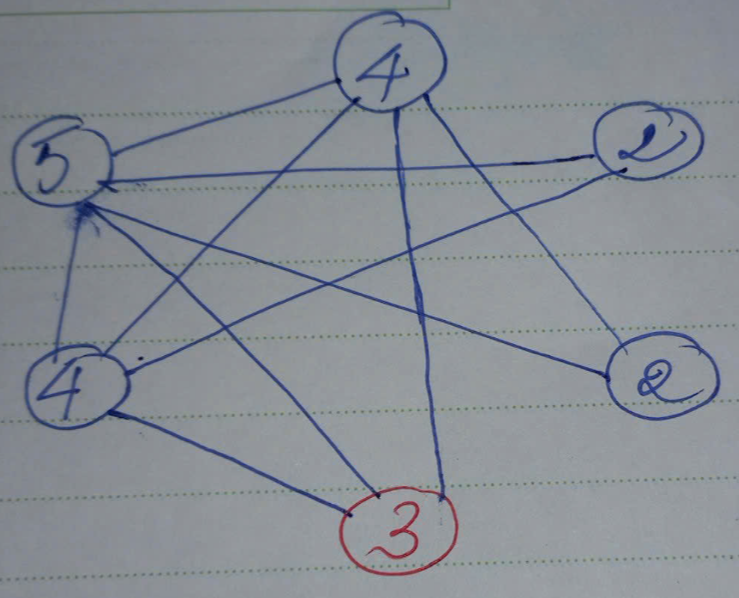
\includegraphics[scale=0.35]{Figures/A_03_01_02.png}
\end{center}

\textbf{Trường hợp 3. }Bậc của đỉnh còn lại bằng 1. Khi đó, dãy bậc của đồ thị là $5,\,4,\,4,\,2,\,2,\,1$, là một dãy graphic. Theo thuật toán Havel-Hakimi, dãy $3,\,3,\,1,\,1,\,0$ và $2,\,0,\,0,\,0$ cũng là các dãy graphic. Tuy nhiên, hiển nhiên không tồn tại đồ thị đơn 4 đỉnh có dãy bậc $2,\,0,\,0,\,0$. Do đó bậc của đỉnh còn lại của đồ thị đã cho không thể bằng 1.

Như vậy bậc của đỉnh còn lại của đồ thị đã cho chỉ có thể là 3. 

\begin{tcolorbox}[breakable]
    \begin{baitoan}[\parencite{shahriari2021invitation}, P10.1.15, p. 368]\label{pb:w02:06}
        Liệu có tồn tại đồ thị đơn mà các đỉnh có bậc là các số nguyên phân biệt? Câu hỏi tương tự cho đồ thị đa.
    \end{baitoan}
\end{tcolorbox}

\textbf{Lời giải. }Giả sử tồn tại đồ thị đơn có $n$ đỉnh thỏa mãn các đỉnh có bậc là các số nguyên phân biệt, ký hiệu các đỉnh là $v_0,\,v_1,\,\ldots,\,v_{n-1}$. Khi đó bậc của mỗi đỉnh sẽ thuộc tập $\{0,\,1,\,2,\,\ldots,\,n-1\}$. Tập hợp này có $n$ phần tử, mà mỗi đỉnh trong đồ thị phải có bậc là các số nguyên phân biệt nên $\deg(v_i) = i$ với mọi $i$. Khi đó, đỉnh $v_{n-1}$ có bậc là $n-1$ nên sẽ nối với tất cả các đỉnh còn lại, đỉnh $v_0$ có bậc là 0 nên không nối với đỉnh nào, điều này mâu thuẫn. Như vậy không tồn tại đồ thị đơn thỏa mãn đề.

Đối với đồ thị đa, câu trả lời là khẳng định. Thật vậy, chẳng hạn xét đồ thị đa có 4 đỉnh như hình bên dưới, khi đó bậc của các đỉnh lần lượt là $1,\,2,\,3,\,4$. 

\begin{center}
    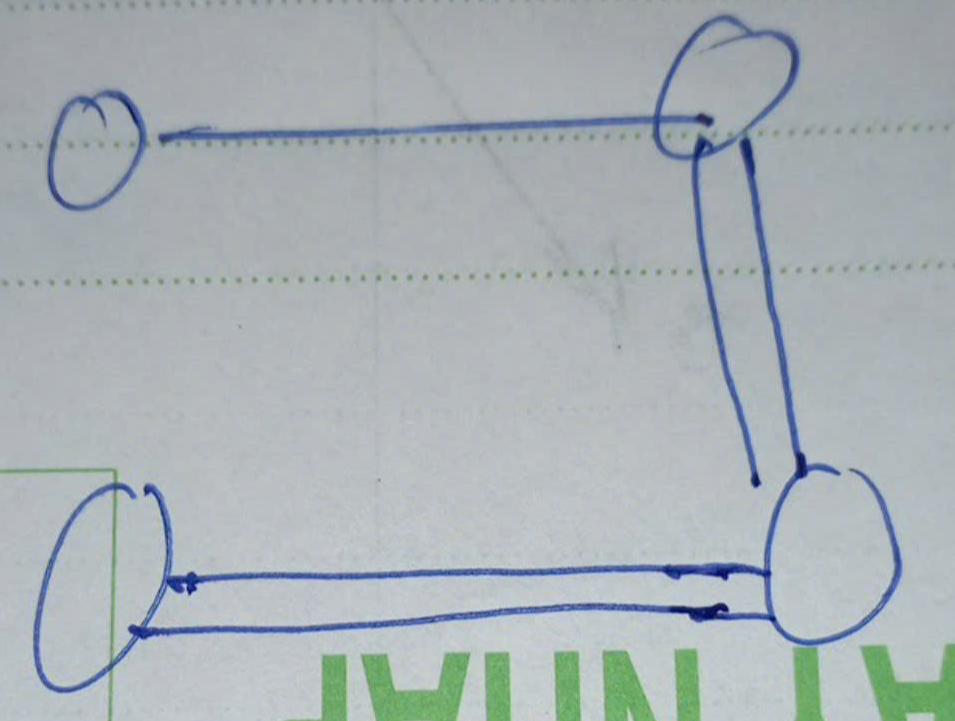
\includegraphics[scale=0.3]{Figures/A_03_01_01.png}
\end{center}

\begin{tcolorbox}[breakable]
    \begin{baitoan}[\parencite{shahriari2021invitation}, P10.1.16, p. 368]\label{pb:w02:05}
        Xét đồ thị đơn $G$ có 94 đỉnh. Giả sử rằng tất cả các đỉnh của $G$ đều có bậc là số lẻ. Chứng minh rằng tồn tại ít nhất ba đỉnh có cùng bậc.
    \end{baitoan}
\end{tcolorbox}

\textbf{Lời giải. }Ta sẽ chứng minh cho trường hợp tổng quát với đồ thị $G$ có $2n$ đỉnh. Do $G$ là đồ thị đơn nên bậc của mỗi đỉnh sẽ thuộc tập $\{0,\,1,\,2,\,\ldots,\,2n-1\}$. Mặt khác, tất cả các đỉnh của $G$ đều có bậc lẻ nên bậc của mỗi đỉnh sẽ thuộc tập $U = \{1,\,3,\,5,\,\ldots,\,2n-1\}$. Giả sử chỉ có tối đa hai đỉnh có cùng bậc, thì khi đó mỗi phần tử trong $U$ sẽ có đúng 2 đỉnh nhận làm bậc, suy ra dãy bậc của đồ thị $G$ sẽ là $$2n-1,\,2n-1,\,2n-3,\,2n-3,\,\ldots,\,3,\,3,\,1,\,1.$$

Áp dụng thuật toán Havel-Hakimi, khi đó dãy $$2n-2,\,2n-4,\,2n-4,\,\ldots,\,2,\,2,\,0,\,0$$ phải là một dãy graphic. Tuy nhiên, không tồn tại đồ thị đơn có $2n-1$ đỉnh thỏa mãn tồn tại một đỉnh có bậc $2n-2$ và một đỉnh có bậc $0$. Như vậy, có ít nhất ba đỉnh trong $G$ có cùng bậc.

\begin{tcolorbox}[breakable]
    \begin{baitoan}\label{pb:w08:01}
        Cho $G = (V,\,E)$ là đồ thị tổng quát với $d_1,\,\ldots,\,d_p\in\mathbb{N}$ là bậc của các đỉnh. Chứng minh: Bậc cao nhất $d_{\max}\coloneqq\max_{1\le i\le p} d_i$ thỏa $d_{\max}\ge\dfrac{2|E|}{|V|}$.
    \end{baitoan}
\end{tcolorbox}

\textbf{Lời giải. }Theo định lý Euler thì $d_1 + d_2 + \cdots + d_p = 2|E|$. Vì $d_{\max} \geq d_i,\,\forall i$ nên $2|E| \leq p\cdot d_{\max} = |V| \cdot d_{\max}$. Suy ra $d_{\max} \geq \dfrac{2|E|}{|V|}$.


% \begin{tcolorbox}[breakable]
%     \begin{baitoan}[\cite{shahriari2021invitation}, P10.1.17, p. 368]\label{pb:w08:02}
%         Giả sử rằng $a_1\ge a_2\ge\cdots a_n$ là một dãy graphic. Chứng minh rằng với mọi $1 \leq k \leq n$ thì 
%         \begin{equation*}
%             \sum_{i=1}^k a_i\le k(k - 1) + \sum_{i=k+1}^n \min\{k,\,a_i\}.
%         \end{equation*}
%     \end{baitoan}
% \end{tcolorbox}

% \textbf{Lời giải. }

% \begin{tcolorbox}[breakable]
%     \begin{baitoan}[\cite{shahriari2021invitation}, P10.1.18, p. 368]\label{pb:w08:03}
%         Xét $p,\,t\in\mathbb{N}^\star$ với $2\le t < p$. Giả sử rằng $a_1\ge a_2\ge\cdots\ge a_{t-1} > a_t\ge\cdots\ge a_{p-1} > a_p$ là dãy bậc của một đồ thị đơn. Chứng minh rằng $a_1\ge a_2\ge\cdots\ge a_{t-1}\ge a_t + 1\ge\cdots\ge a_{p-1}\ge a_p + 1$ cũng là dãy bậc của một đồ thị đơn.
%     \end{baitoan}
% \end{tcolorbox}

% \textbf{Lời giải. }

% \begin{tcolorbox}[breakable]
%     \begin{baitoan}[\cite{shahriari2021invitation}, P10.1.19, pp. 368--369]\label{pb:w08:04}
%         Tồn tại hay không đồ thị đơn với $48$ đỉnh, trong đó tập hợp bậc của các đỉnh là $\{4,\,7,\,47\}$? Tổng quát, xét $S = \{a_1,\,\ldots,\,a_n\}$ là tập hợp khác rỗng gồm $n$ số nguyên dương với $a_1 < a_2 < \cdots < a_n$. Chứng minh rằng tồn tại đồ thị đơn $G$ với $a_n + 1$ đỉnh, trong đó tập hợp bậc của các đỉnh chính là $S$. 
%     \end{baitoan}
% \end{tcolorbox}

% \textbf{Lời giải. }
    \section{Lý thuyết Ramsey}
      \subsection{Định lý Ramsey}
      \subsection{Số Ramsey}
    \section{Ứng dụng trong Lập trình thi đấu}
      % \subsection{Hàm sinh trong lập trình thi đấu}
  \newpage

  % \addtocontents{toc}{\protect\newpage}
  % \part{Giải tích}
  %   \setcounter{section}{0}
  %   \setcounter{baitoan}{0}
  %   \section{Dãy số}
  %     \subsection{Cấp số cộng \& Cấp số nhân}
  %     \subsection{Giới hạn dãy số}

\begin{tcolorbox}[breakable]
    \begin{baitoan}
        Tính $\lim\limits_{n\to+\infty} \dfrac{an + b}{cn + d}$ theo $a,\,b,\,c,\,d \in \mathbb{R},\, (c,\,d) \ne (0,\,0)$.
    \end{baitoan}
\end{tcolorbox}

\textbf{Lời giải. }

Không mất tính tổng quát, giả sử $c > 0$. Ta có $$\left|\dfrac{an+b}{cn+d} - \dfrac{a}{c}\right|  = \left|\dfrac{acn + be - acn - ad}{c(cn+d)}\right| = \left|\dfrac{bc-ad}{c(cn+d)}\right|.$$ 

Lấy $\varepsilon > 0$ bất kỳ, ta có $\left|\dfrac{an+b}{cn+d} - \dfrac{a}{c}\right| < \varepsilon \iff \left|\dfrac{bc-ad}{c(cn+d)}\right| < \varepsilon \iff \left|c(cn+d)\right| > \dfrac{\left|bc-ad\right|}{\varepsilon} \iff \left|cn+d\right| > \dfrac{\left|bc-ad\right|}{c\varepsilon} \Longleftarrow cn + d > \dfrac{\left|bc-ad\right|}{c\varepsilon} \Longleftarrow n > \dfrac{\left|bc-ad\right|}{\varepsilon} - \dfrac{d}{c}$.

Suy ra nếu chọn $N_\varepsilon = \left\lfloor\dfrac{\left|bc-ad\right|}{\varepsilon} - \dfrac{d}{c}\right\rfloor+1$ thì $\left|\dfrac{an+b}{cn+d} - \dfrac{a}{c}\right| < \varepsilon$ với mọi $n \geq N_\varepsilon$. Theo định nghĩa suy ra $\lim\limits_{n\to+\infty} \dfrac{an + b}{cn + d} = \dfrac{a}{c}$.




\begin{tcolorbox}[breakable]
    \begin{baitoan}
        Tính $\lim\limits_{n\to+\infty} \dfrac{P(n)}{Q(n)}$ với 
        \begin{enumerate}
            \item[(a)] $P,\,Q \in \mathbb{R}[x],\,Q \not\equiv 0$;
            \item[(b)]$P,\,Q \in \mathbb{C}[x],\,Q \not\equiv 0$.
        \end{enumerate}
    \end{baitoan}
\end{tcolorbox}

\textbf{Lời giải. }
  %   \section{Hàm số}
  %     \subsection{Giới hạn hàm số}
  %     \subsection{Hàm số liên tục}
  %   \section{Đạo hàm}
  %     \subsection{Đạo hàm}
  %     \subsection{Xấp xỉ đạo hàm}
  %   \section{Tích phân}
  %     \subsection{Tích phân}
  %     \subsection{Xấp xỉ tích phân}
  %   \section{Kết hợp Dãy số, Vi phân và Tích phân}
  %     \begin{baitoan}
    Cho
\end{baitoan}
  % \newpage

  \printbibliography[title={Tài liệu}]
\end{document}

%%%%%%%%%%%%%%%%%%%%
%%% Some useful codes
% 1. Mathematical equation
  % \begin{align}
  % X &= Y+Z \tag*{Because $X=C$} \\
  % Y &= X-Z \tag*{Rearranging}
  % \end{align}
  % \tag{} \eqref{}
%%%%%%%%%%%%%%%%%%%%